% Notes:
% 
% Use 'named destinations' to open a PDF at a specified location.  These are
% not the same as bookmarks or links.  One could also use 'PDF Open parameters':
%
%   http://partners.adobe.com/public/developer/en/acrobat/PDFOpenParameters.pdf

\documentclass{article}

\usepackage[utf8]{inputenc}  % utf8 om de letters é en dergelijke te kunnen gebruiken
\usepackage{amsmath}
\usepackage{amssymb}
\usepackage{graphicx}
\usepackage{color}
\usepackage[dutch]{babel}
\usepackage{hyperref}
\usepackage{pgf,tikz}
\usetikzlibrary{arrows}


\graphicspath{{graphics/}}

\title{USolv-IT formularium}

\newcommand{\Z}{\mathbb{Z}}
\newcommand{\R}{\mathbb{R}}
\newcommand{\N}{\mathbb{N}}
\newcommand{\Q}{\mathbb{Q}}
\newcommand{\C}{\mathbb{C}}

\newcommand{\ds}{\displaystyle}
\newcommand{\Frac}[2]{\frac{\ds #1}{\ds #2}}
\newcommand{\degree}{\ensuremath{^\circ}}
\newcommand{\rad}{\ensuremath{\mbox{ rad}}}
\newcommand{\dx}{\ensuremath{\,dx}}

\DeclareMathOperator{\arccot}{arccot}

\begin{document}

\maketitle

\tableofcontents

\hypertarget{combinatoriek}{}
\section{COMBINATORIEK} \label{combinatoriek}

\hypertarget{telproblemen}{}
\subsection{Telproblemen} \label{telproblemen}

\hypertarget{variaties}{}
\subsubsection{Variaties} \label{variaties}
\begin{itemize}
\item \textcolor{green}{Wat?}\newline
Een variatie van $p$ elementen uit $n$ elementen $(p\leq n )$ is een {\bf geordend} $p$-tal van $p$ {\bf verschillende } elementen gekozen uit een gegeven verzameling van $n$ elementen.
\item \textcolor{green}{Voorbeeld.} \newline
Enkele variaties van 3 elementen uit$\{a, b, c, d\}$ zijn $abc, abd, acb, acd, \ldots$
\item \textcolor{green}{Formule.} \newline
Het aantal variaties van $p$ elementen uit $n$ elementen $(1\leq p\leq n)$:
\[V^p_n = \displaystyle \Frac{n!}{(n-p)!}\]
\end{itemize}

\hypertarget{herhalingsvariaties}{}
\subsubsection{Herhalingsvariaties} \label{herhalingsvariaties}
\begin{itemize}
\item \textcolor{green}{Wat?} \newline
Een herhalingsvariatie van $p$ elementen uit $n$ elementen is een {\bf geordend} $p$-tal van elementen gekozen uit een gegeven verzameling van $n$ elementen. Eenzelfde element mag meer dan eens voorkomen!
\item \textcolor{green}{Voorbeeld.} \newline
Enkele herhalingsvariaties van 3 elementen uit $\{a, b, c, d\}$ zijn $aaa, aab, abc, aba, acc, \ldots$
\item \textcolor{green}{Formule.} \newline
Het aantal herhalingsvariaties van $p$ elementen uit $n$ elementen is:
\[\bar{V}^p_n=n^p\]
\end{itemize}

\hypertarget{permutaties}{}
\subsubsection{Permutaties} \label{permutaties}
\begin{itemize}
\item \textcolor{green}{Wat?} \newline
Een permutatie van $n$ verschillende elementen is een variatie van $n$ elementen uit $n$ elementen.
\item \textcolor{green}{Voorbeeld.} \newline
Alle permutaties van 3 elementen uit $\{a, b, c\}$ zijn $abc, acb, bac, bca, cab, cba$.
\item \textcolor{green}{Formule.} \newline
Het aantal permutaties van $n$ elementen is:
\[P_n=n!\]
\end{itemize}

\hypertarget{herhalingspermutaties}{}
\subsubsection{Herhalingspermutaties} \label{herhalingspermutaties}
\begin{itemize}
\item \textcolor{green}{Wat?} \newline
Herhalingspermutaties zijn permutaties van $n$ elementen waarbij onder de $n$ elementen dezelfde elementen meerdere malen mogen voorkomen.
\item \textcolor{green}{Voorbeeld.} \newline
Enkele herhalingspermutaties van ${a, a, b, c}$ zijn $aabc, abca, abac,\ldots$.
\item \textcolor{green}{Formule.} \newline
Stel $l_i$ het aantal keer dat elk van de $p$ verschillende elementen $a_i$ voorkomt en $n$ het totaal aantal elementen, dan is het aantal herhalingspermutaties van die $n$ elementen:
\[\bar{P}^{l_1,l_2,\ldots,l_p}_n=\displaystyle\Frac{n!}{l_1!l_2!\ldots l_p!}\]
\end{itemize}

\hypertarget{combinaties}{}
\subsubsection{Combinaties} \label{combinaties}
\begin{itemize}
\item \textcolor{green}{Wat?} \newline
Een combinatie van $p$ elementen uit $n$ elementen $(p \leq n)$ is een deelverzameling van $p$ elementen gekozen uit een gegeven verzameling van $n$ elementen. De volgorde is niet van belang!
\item \textcolor{green}{Voorbeeld.} \newline
Alle combinaties van 3 elementen uit $\{a, b, c, d\}$ zijn: $\{a, b, c\}, \{a, b, d\}, \{a, c, d\}, \{b, c, d\}$
\item \textcolor{green}{Formule.} \newline
Het aantal combinaties van $p$ elementen uit $n$ elementen is:
\[C^p_n=\displaystyle\Frac{n!}{p!(n-p)!}\]
\end{itemize}

\hypertarget{herhalingscombinaties}{}
\subsubsection{Herhalingscombinaties} \label{herhalingscombinaties}
\begin{itemize}
\item \textcolor{green}{Wat?}\newline
Herhalingscombinaties zijn combinaties van $p$ elementen uit $n$ elementen waarbij onder de $n$ elementen dezelfde elementen meerdere malen mogen voorkomen.
\item \textcolor{green}{Voorbeeld.} \newline
Enkele herhalingscombinaties van 7 elementen uit $\{a, a, a, b, b, b, c, c, c\}$ zijn $\{a, a, a, b, b, b, c\}, \{a, a, b, b, b, c, c\}, \ldots$
\item \textcolor{green}{Formule.} \newline
Het aantal herhalingscombinaties van $p$ elementen uit $n$ elementen is:
\[\bar{C}^p_n=C^p_{n+p-1}\]
\end{itemize}

\hypertarget{aantal_deelverzamelingen}{}
\subsubsection{Aantal deelverzamelingen van een verzameling} \label{aantal_deelverzamelingen}

Het aantal deelverzamelingen van een verzameling met $n$ elementen is $2^n$. 

\hypertarget{duivenhokprincipe}{}
\subsubsection{Het duivenhokprincipe} \label{duivenhokprincipe}

Worden er $n$ voorwerpen geplaatst in $r$ laden, met $n>r$, dan is er minstens \'e\'en lade die minstens twee voorwerpen bevat.

\hypertarget{binomium}{}
\subsubsection{Het binomium van Newton} \label{binomium}

In onderstaande formules wordt volgende notatie gebruikt:
\[\left( \begin{array}{c}n\\p \end{array} \right)=\displaystyle \Frac{n!}{p!(n-p)!}\]
Dit noemen we de binomiaalco\"effici\"enten.\newline
\textcolor{green}{De binomiaalformule:}
\[(a+b)^n=\left( \begin{array}{c}n\\0 \end{array} \right)a^n + \left( \begin{array}{c}n\\1 \end{array} \right)a^{n-1}b + \left( \begin{array}{c}n\\2 \end{array} \right)a^{n-2}b^2+\ldots + \left( \begin{array}{c}n\\n-1 \end{array} \right)ab^{n-1}+\left( \begin{array}{c}n\\n \end{array} \right)b^n \]
Of ook nog:
\[(a+b)^n=\sum_{i=0}^n \left( \begin{array}{c}n\\i \end{array} \right)a^{n-i}b^i\]


\hypertarget{kansrekenen}{}
\subsection{Kansrekening} \label{kansrekenen}

\hypertarget{laplace}{}
\subsubsection{Formule van Laplace} \label{laplace}

Voor volgende formules is het belangrijk de begrippen {\it uitkomstenverzameling} en {\it gebeurtenis} te begrijpen.
\begin{itemize}
\item Een \textcolor{green}{uitkomstenverzameling (universum)} is de verzameling van alle mogelijke uitkomsten bij een kansexperiment, bv. bij een dobbelsteen : $U =\{1, 2, 3, 4, 5, 6\}$.
\item Een \textcolor{green}{gebeurtenis} is een deelverzameling van de uitkomstenverzameling, bij het voorbeeld van de dobbelsteen zijn $\{6\}, \{1, 2, 4\}$ mogelijke gebeurtenissen.
\end{itemize}
\textcolor{green}{De formule van Laplace:}\newline
Stel $n$ het aantal elementen van het universum $U$ en $p$ het aantal elementen van de gebeurtenis $A$, dan is de kans voor de gebeurtenis ($P(A)$):\newline\newline
\[P(A)=\displaystyle \Frac{p}{n}\]\newline
Zo is bv. de kans om met een dobbelsteen 3 of 4 te gooien : $P(\{3,4\})= \displaystyle{ \Frac{2}{6}=\Frac{1}{3}}.$\newline\newline\newline

\hypertarget{kanswetten}{}
\subsubsection{Belangrijke kanswetten} \label{kanswetten}

\begin{itemize}
\item Zekere gebeurtenis: $P(U)=1$
\item Onmogelijke gebeurtenis: $P(\emptyset)=0$
\item Zij $\bar A$ (=$U\backslash A$)  het complement van de gebeurtenis $A$ , dan geldt: \[P(A)+P(\bar A)=1\]
\item Zij $A$ en $B$ twee gebeurtenissen, dan geldt: \[P(A\cup B)=P(A) +P(B)-P(A\cap B)\]
\item Gevolg: als $A$ en $B$ disjuncte gebeurtenissen zijn $(A\cap B=\emptyset)$, dan geldt: \[P(A\cup B)=P(A) + P(B)\]
\item Samengestelde experimenten:
\begin{description}
\item [(i)] Afhankelijke deelexperimenten / voorwaardelijke kans:\vskip 0.5cm
\textcolor{green}{Voorbeelden:} Je trekt, zonder teruglegging van de kaarten, twee kaarten uit een spel. Hoe groot is de kans dat je als eerste kaart een harten trekt en als tweede kaart een klaveren?\vskip 0.5cm
\textcolor{green}{Formule:} Stel $p(A\:|\:B)$ de voorwaardelijke kans van A als B reeds gerealiseerd is, dan geldt: \[P(A\cap B)= P(B)\cdot P(A\:|\:B)\]
Uitbreiding: \[P(A\cap B\cap C)=P(A)\cdot P(B\:|\:A)\cdot P(C\:|\:A\cap B)\]
Het voorbeeld wordt dus: $P=\displaystyle\Frac{13}{52}\cdot \displaystyle\Frac{13}{51}$
\item[(ii)] Onafhankelijke deelexperimenten:\vskip 0.5cm
\textcolor{green}{Voorbeelden:} Je trekt, met teruglegging van de kaarten, twee kaarten uit een spel. Wat is de kans dat de eerste kaart een harten is en de tweede een klaveren?
\vskip 0.5cm
\textcolor{green}{Formule:} Zij $A$ en $B$ onafhankelijke gebeurtenissen, dan geldt:
\[P(A\cap B)=P(A)\cdot P(B)\] 
Het voorbeeld wordt dus: $P=\displaystyle\Frac{13}{52}\cdot \displaystyle\Frac{13}{52}$
\end{description}
\end{itemize}


% Dit werk is gelicenseerd onder een Creative Commons
% Naamsvermelding-GelijkDelen 3.0 Unported.
% Bezoek http://creativecommons.org/licenses/by-sa/3.0/ om een kopie te zien 
% van de licentie of stuur een brief naar Creative Commons, 444 Castro Street, 
% Suite 900, Mountain View, California, 94041, USA.

\hypertarget{analyse}{}
\section{ANALYSE} \label{analyse}

\hypertarget{relaties}{}
\subsection{Soorten relaties} \label{relaties}

\begin{enumerate}
\item {\bf Relatie: } Een relatie van $A$ naar $B$ is een verzameling van koppels waarvan het eerste element tot $A$ behoort en het tweede tot $B$.
\item {\bf Functie: } Een \hypertarget{functie}{functie} van $A$ naar $B$ is een relatie van $A$ naar $B$ waarbij elk element van $A$ hoogstens \'e\'en beeld heeft.\label{functie}
\item {\bf Afbeelding: } Een afbeelding  van $A$ in $B$ is een relatie van $A$ naar $B$ waarbij elk element van $A$ juist \'e\'en beeld heeft .
\item {\bf Injectie: } Een injectie van $A$ in $B$ is een relatie van $A$ naar $B$ waarbij elk element van $A$ juist \'e\'en beeld heeft en elk element van $B$ het beeld is van hoogstens \'e\'en element van $A$.
\item {\bf Surjectie: } Een surjectie van $A$ op $B$ is een afbeelding van $A$ in $B$ waarbij elk element van $B$ het beeld is van minstens \'e\'en element van $A$.
\item {\bf Bijectie: } Een bijectie van $A$ op $B$ is een afbeelding van $A$ in $B$ waarbij elk element van $B$ het beeld is van juist \'e\'en element van $A$.
\end{enumerate}

\hypertarget{reele_functies}{}
\subsection{Re\"ele functies} \label{reele_functies}

\hypertarget{parameters}{}
\subsubsection{Invloed van parameters op de grafiek van een functie} \label{parameters}

Zij een functie $f(x)$ gegeven en beschouwen we de functies $af(x-\alpha)+\beta$ 		waarbij $a, \alpha$ en $\beta$ parameters zijn. Dan hebben de verschillende 		parameters volgende invloed op de grafiek van $f(x)$:\newline
\begin{itemize}
\item $\alpha :$ verschuiving in de richting van de $X$-as over $|\alpha|$ 		\'e\'enheden:\newline
	\begin{itemize}
	\item[*] naar rechts: als $\alpha$ positief is
	\item[*] naar links: als $\alpha$ negatief is
	\end{itemize}
\item $\beta :$ verschuiving in de richting van de $Y$-as over $|\beta|$ 		\'e\'enheden:\newline
	\begin{itemize}
	\item[*] naar boven: als $\beta$ positief is
	\item[*] naar onder: als $\beta$ negatief is
	\end{itemize}
\item $a :$ `uitrekking' van de grafiek met factor $|a|$
\end{itemize}

\hypertarget{eerstegraadsfuncties}{}
\subsubsection{Eerstegraadsfuncties} \label{eerstegraadsfuncties}

\begin{itemize}
  \item \textcolor{green}{Vorm.}
    \[
      f: x\mapsto ax+b \;\;\;\mbox{met}\: a\neq 0
    \]
  \item \textcolor{green}{Grafiek.}\newline
    Een rechte waarbij $a$ de richtingsco\"effici\"ent is en $b$ het stuk afgesneden op de $y$-as.
    \begin{center}
    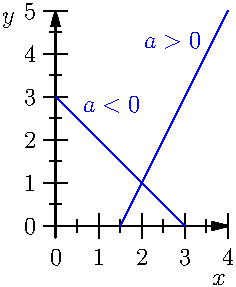
\includegraphics{rechten.pdf}
    \end{center}
    Als $a>0$, is de rechte stijgend.\newline
    Als $a<0$, is de rechte dalend.\newline
    Het snijpunt met de $X$-as is $(-\ds\Frac{b}{a}, 0)$ en met de $Y$-as $(0, b)$
  \item \textcolor{green}{Formules.}\newline
    Indien twee punten van de rechte $(x_1, y_1)$ en $(x_2, y_2)$ gegeven zijn, is de {\bf richtingsco\"effici\"ent}:
    \[a=\ds\Frac{y_2-y_1}{x_2-x_1}\]
    De \hypertarget{vgl_rechte}{vergelijking van de rechte} is dan:
    \[
      y-y_1=a(x-x_1)
    \]\label{vgl_rechte}
  \item \textcolor{green}{Tekenverloop.}\newline
    \begin{tabular}{c|ccccc}
    $x$ & $-\infty$ & & $-\ds\Frac{b}{a}$ & & $+\infty$\\
    \hline
    $ax+b$ & & tegengesteld teken van $a$ & 0 & teken van $a$ & \\		
    \end{tabular}
\end{itemize}

\hypertarget{tweedegraadsfuncties}{}
\subsubsection{Tweedegraadsfuncties} \label{tweedegraadsfuncties}
		\begin{itemize}%tweedegraadsfuncties
		\item \textcolor{green}{Vorm.}
		\[f: x\mapsto ax^2+bx+c \;\;\;\mbox{met}\: a\neq 0\]
		\item \textcolor{green}{Grafiek.}\newline
		Een \hypertarget{parabool}{{\bf parabool}}, waarbij $a$ de aard van de parabool aangeeft:\label{parabool}\newline
		als $a>0$, dan is de holle kant naar boven (dalparabool)\newline 
		%\docLink[tekening]{dalparabool.jpg}{\includegraphics{tekening.gif}}\newline
                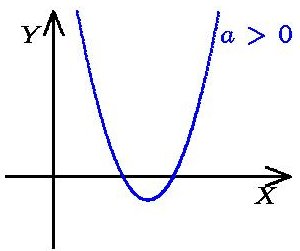
\includegraphics{dalparabool.jpg}
		als $a<0$, dan is de holle kant naar beneden (bergparabool)\newline
		%\docLink[tekening]{bergparabool.jpg}{\includegraphics{tekening.gif}}\newline
                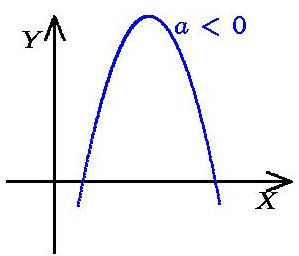
\includegraphics{bergparabool.jpg}
		Verder geldt dat $|a|$ de 'uitrekkingsfactor' voorstelt van de parabool t.o.v. de 		standaardparabool: $P\:\leftrightarrow\: y=x^2$.
		\item \textcolor{green}{Formules.}\newline
		De \hypertarget{topvergelijking}{{\bf top} van de parabool} wordt gegeven door:\label{topvergelijking}
		\[t\:(-\ds\Frac{b}{2a},\ds\Frac{4ac-b^2}{4a}) \]
		en de {\bf symmetrie-as}:
		\[S\:\leftrightarrow\:x=-\ds\Frac{b}{2a}\]
		De {\bf topvergelijking} van de parabool met top $t\:(\alpha, \beta)$
		\[P\:\leftrightarrow\: y=a(x-\alpha)^2+\beta\]
		%\docLink[tekening]{parabool.jpg}{\includegraphics{tekening.gif}}\newline
                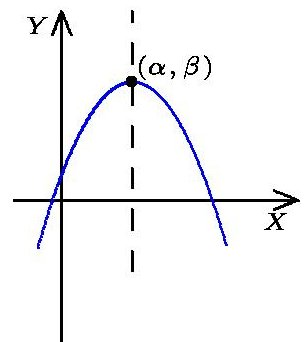
\includegraphics{parabool.jpg}
		\item \textcolor{green}{Tekenverloop.}\newline
		Stel $x_i$ de eventuele nulpunten van de functie $f:x\:\mapsto \:ax^2+bx+c$. 
		De discriminant wordt gegegeven door volgende formule: 
		\[b^2-4ac\]
		en de nulpunten zijn dan
		\[x_{1, 2}=\displaystyle\Frac{-b\pm\sqrt{b^2-4ac}}{2a}\]
		\begin{itemize}%tekenverloop
		\item[*] Discriminant  $>0$\vskip 0.5cm
		\begin{tabular}{c|ccccccc}
		$x$ & $-\infty$ & & $x_1$ & & $x_2$ & & $+\infty$\\
		\hline
		$ax^2+bx+c$ & & teken van $a$ & 0& tegengesteld teken van $a$ & 0 & teken van $a$ 		&\\ 	
		\end{tabular}\vskip 1cm
		\item[*] Discriminant $=0$\vskip 0.5cm
		\begin{tabular}{c|ccccc}
		$x$ & $-\infty$ & & $x_1=x_2$ & & $+\infty$\\
		\hline
		$ax^2+bx+c$ & & teken van $a$ & 0 & teken van $a$ & \\		
		\end{tabular}\vskip 1cm
		\item[*] Discriminant $<0$\vskip 0.5cm
		\begin{tabular}{c|ccc}
		$x$ & $-\infty$ &  & $+\infty$\\
		\hline
		$ax^2+bx+c$ & & teken van $a$ & \\		
		\end{tabular}
		\end{itemize}%tekenverloop
		\end{itemize}%tweedegraadsfuncties

\hypertarget{veeltermfuncties}{}
\subsubsection{Veeltermfuncties} \label{veeltermfuncties}
		\begin{itemize}%veeltermfuncties
		\item \textcolor{green}{Vorm.}
		\[f:x\, \mapsto \: a_nx^n+a_{n-1}x^{n-1}+\ldots +a_1x+a_0\:\mbox{met} \:a_n\neq 0\]
		\item \textcolor{green}{Formules.}\newline
		\hypertarget{euclidische_deling}{{\bf Euclidische deling:}}\label{euclidische_deling} zij $f(x), d(x) \neq 0 \in\R 		[x]$ dan bestaat er juist \'e\'en $q(x)$ en $r(x) \in\R [x]$ zodat geldt:
		 \[f(x)=d(x)\cdot q(x)+r(x)\:\:\mbox{met 		graad}(r(x))<\:\mbox{graad}(d(x))\:\mbox{of}\:r(x)=0\]\newline
		{\bf Praktisch voorbeeld}\newline
		%\docLink[tekening]{euclid.jpg}{\includegraphics{tekening.gif}}\newline
                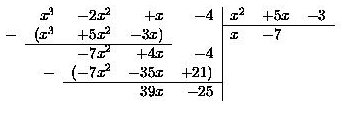
\includegraphics{euclid.jpg}

		\hypertarget{reststelling}{{\bf Reststelling:}}\label{reststelling} De rest van een deling van $f(x)$ door $x-a$ 		is gelijk aan $f(a)$\newline\newline
		{\bf Criterium van deelbaarheid:} \[x-a \: |\: f(x)\:\Leftrightarrow\: f(a)=0\]
		\hypertarget{merkwaardige_quotienten}{{\bf Enkele stellingen:}}\label{merkwaardige_quotienten} 
		\begin{itemize}
		\item[*]Het verschil van twee gelijknamige machten is deelbaar door het verschil van 		de grondtallen.
		\[x^n-a^n=(x-a)(x^{n-1}+ax^{n-2}+a^2x^{n-3}+\ldots+a^{n-2}x+a^{n-1})\]
		\item[*]De som van twee gelijknamige {\it oneven} machten is deelbaar door de som 		van de grondtallen.
		\[x^{2n+1}+a^{2n+1}=(x+a)(x^{2n}-ax^{2n-1}+a^2x^{2n-2}-\ldots-a^{2n-1}x+a^{2n})\]
		\end{itemize}
		{\bf Methode van Horner:} zie %\docLink[formularium]{form_algebra.tex}[n-de graadsvergelijkingen]{$n$-de graadsvergelijkingen}
		\end{itemize}%veeltermfuncties

\hypertarget{rationale_functies}{}
\subsubsection{Gebroken rationale functies} \label{rationale_functies}
			\begin{itemize}%gebroken rationale functies
			\item\textcolor{green}{Vorm.}\newline
			\[f:x\mapsto \ds\Frac{g(x)}{h(x)} \:\mbox{met g(x) en h(x) veeltermen 			en graad}(h(x))\geq 1\]
			\item \textcolor{green}{Kenmerken.}\newline
				\begin{itemize}
				\item[*] domein: $\:\R \backslash h^{-1}\{0\}$
				\item[*] $f^{-1}\{0\}=g^{-1}\{0\}\cap \:\mbox{domein}\:f$
				\end{itemize} 
			\end{itemize}%gebroken rationale functies

\hypertarget{goniometrische_functies}{}
\subsubsection{Goniometrische functies} \label{goniometrische_functies}

\begin{itemize}
\item \textcolor{green}{\hypertarget{periodieke_functies}{Periodieke functies}}\label{periodieke_functies}\newline
Een functie is een {\bf periodieke functie} als en slechts als er een getal $\omega \in \R_0$ bestaat zodat \[\forall x \in \:\mbox{dom}f : f(x+\omega)=f(x).\] Het 		kleinste positief getal $\omega$ waarvoor dit geldt, noemen we de {\bf periode} van 		de functie.
\item \textcolor{green}{Elementaire goniometrische functies}\newline\newline
\hypertarget{sinusfunctie}{{\bf De sinusfunctie: }}\label{sinusfunctie}$f :x\mapsto\sin x$\vskip 0.5cm

Kenmerken: \begin{itemize}
		\item[*] domein: $\R$
		\item[*] bereik: $[-1, 1]$
		\item[*] $f^{-1}\{0\}=\{k\pi\:|\:k\in\Z\}$
		\item[*] periode: $2\pi$
		\item[*] grafiek %\docLink[tekening]{sinus.jpg}{\includegraphics{tekening.gif}}\newline
                         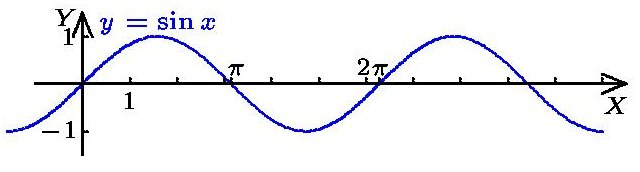
\includegraphics{sinus.jpg}
		\end{itemize}
\hypertarget{cosinusfunctie}{{\bf De cosinusfunctie: }}\label{cosinusfunctie}$f :x\mapsto\cos x$\vskip 0.5cm

Kenmerken: \begin{itemize}
		\item[*] domein: $\R$
		\item[*] bereik: $[-1, 1]$
		\item[*] $f^{-1}\{0\}=\{(2k+1)\ds\Frac{\pi}{2}\:|\:k\in\Z\}$
		\item[*] periode: $2\pi$
		\item[*] grafiek %\docLink[tekening]{cosinus.jpg}{\includegraphics{tekening.gif}}\newline
                         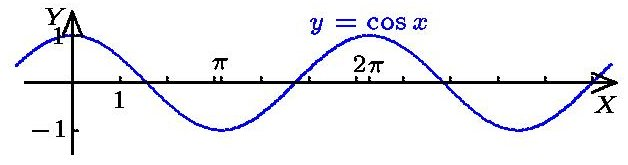
\includegraphics{cosinus.jpg}
		\end{itemize}
\hypertarget{tangensfunctie}{{\bf De tangensfunctie: }}\label{tangensfunctie}$f :x\mapsto\tan{x}$\vskip 		0.5cm
Kenmerken:\begin{itemize}
		\item[*] domein: $\R \backslash \{(2k+1)\ds\Frac{\pi}{2}\:|\:k\in\Z\}$
		\item[*] bereik: $\R$
		\item[*] $f^{-1}\{0\}=\{k\pi\:|\:k\in\Z\}$
		\item[*] periode: $\pi$
		\item[*] grafiek 
		\end{itemize}
		%\docLink[tekening]{tangens.jpg}{\includegraphics{tekening.gif}}\newline
                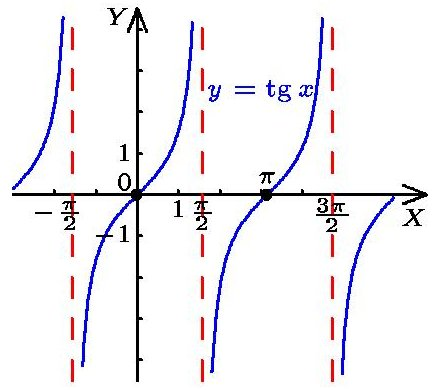
\includegraphics{tangens.jpg}

\hypertarget{}{{\bf De cotangensfunctie: }}\label{cotangensfunctie}$f :x\mapsto\mbox{cotg}x$
\vskip 0.5cm
Kenmerken:\begin{itemize}
		\item[*] domein: $\R \backslash \{k \pi\:|\:k\in\Z\}$
		\item[*] bereik: $\R$
		\item[*] $f^{-1}\{0\}=\{(2k+1)\ds\Frac{\pi}{2}\:|\:k\in\Z\}$
		\item[*] periode: $\pi$
		\end{itemize}	

\item \textcolor{green}{\hypertarget{algemene_sinusfunctie}{Algemene sinusfuncties: }}$f:x\:\mapsto\: a\sin(b(x-c))+d$ \label{algemene_sinusfunctie}\newline\newline
Kenmerken:\begin{itemize}
		\item[*] $|a|$ is de amplitude (maximale uitwijking t.o.v. de 				evenwichtsstand)
		\item[*] periode: $\ds\Frac{2\pi}{b}$
		\item[*] domein: $\R$
		\item[*] bereik: $[-|a|+d, |a|+d]$
		\item[*] $c:$ verschuiving in de richting van de $X$-as over $|c|$ 					\'e\'enheden:\newline
			\begin{itemize}
			\item[*] naar rechts: als $c$ positief is
			\item[*] naar links: als $c$ negatief is
			\end{itemize}
		\item[*] $d:$ verschuiving in de richting van de $Y$-as over $|d|$ 					\'e\'enheden:\newline
			\begin{itemize}
			\item[*] naar boven: als $d$ positief is
			\item[*] naar onder: als $d$ negatief is
			\end{itemize}

		\end{itemize}
\item \textcolor{green}{Toepassing: } $f:x\:\mapsto\:a\sin x+b \cos x$
\newline\newline
Methode voor het omvormen tot een algemene sinusfunctie:
\begin{eqnarray*}
f(x) & = & a\sin{x} + b\cos{x}\\
     & = & a(\sin{x} + \frac{b}{a}\cos{x})\\
     &   & \text{Stel } \ds\Frac{b}{a} = \tan{\varphi}\:\text{ met } \:\varphi \in ]0, \ds\Frac{\pi}{2}[ \:\text{ als }\: \ds\Frac{b}{a} > 0 \\
   %  &   & \hskip 1cm \mbox{Stel } $\:\ds\Frac{b}{a}=$tg$\varphi\:\mbox{ met } \:\varphi \in ]0, \ds\Frac{\pi}{2}[ \:\mbox{ als }\: \ds\Frac{b}{a} > 0$  				\\
     &   & \text{en } \varphi \in ]-\ds\Frac{\pi}{2}, 0[ \:\text{ als }\: \ds\Frac{b}{a} < 0 \\
   %  &   & \hskip 4.3 cm $\varphi \in ]-\ds\Frac{\pi}{2}, 0[ \:\mbox{ als }\: \ds\Frac{b}{a} < 0$  \\
     & = & a(\sin{x} + \tan{\varphi}\cos{x})\\
     & = & a(\sin{x} + \frac{\sin{\varphi}}{\cos{\varphi}}\cos{x})\\
     & = & \ds \Frac{a}{\cos\varphi}(\sin x\ \cos \varphi + \sin \varphi \cos{x})\\			
     & = & \ds \Frac{a}{\cos\varphi}\sin(x + \varphi)
\end{eqnarray*}
	\item \textcolor{green}{Formules}\newline 
%Zie \docLink[formularium]{form_goniometrie.tex}[]{Goniometrie.}
\end{itemize}

\hypertarget{exponentiele_functies}{}
\subsubsection{Exponenti\"ele functies} \label{exponentiele functies}
		\begin{itemize}%exponentiele functies
		\item \textcolor{green}{Vorm}\newline
		\[f: x \mapsto a^x \:\mbox{met}\: a\in \R^+_0\backslash \{1\}\]
		\item \textcolor{green}{Kenmerken}
			\begin{itemize}
			\item[*] domein: $\R$
			\item[*] bereik: $\R^+_0$
			\item[*] $f^{-1}\{0\} = \emptyset$
			\end{itemize}
		\item \textcolor{green}{Speciaal geval}\newline
		\[f: x \mapsto e^x \:\mbox{met $e$ het getal van Euler ($e$ = 		2,718281828459$\ldots$)}\]
		\item \textcolor{green}{Grafiek}\newline
		%\docLink[tekening]{exponentieleB.jpg}{\includegraphics{tekening.gif}}
		%\docLink[tekening]{exponentieleA.jpg}{\includegraphics{tekening.gif}}
                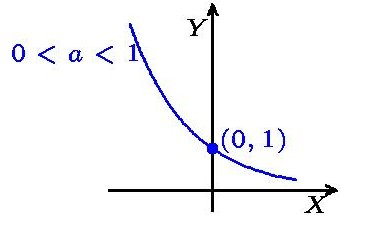
\includegraphics{exponentieleB.jpg}
                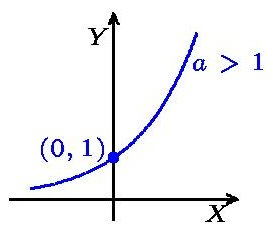
\includegraphics{exponentieleA.jpg}
		\end{itemize}%exponentiele functies

\hypertarget{logaritmische_functies}{}
\subsubsection{Logaritmische functies} \label{logaritmische functies}
		\begin{itemize}%logaritmische functies
		\item  \textcolor{green}{Definitie logaritmen}\newline
		\[\forall a\in \R^+_0\backslash \{1\} : y = \mbox{log}_a x\: \Leftrightarrow\: a^y = 		x\]
		\item \textcolor{green}{Speciale gevallen}\newline
		Briggse logaritme : log $x$ is de logaritme met grondtal $a=10$\newline
		Neperiaanse logaritme: ln $x$ is de logaritme met grondtal $a=e$\newline
		\item \textcolor{green}{Vorm}
		\[f:x\mapsto \mbox{log}_a x \: \mbox{met}\: a\in \R^+_0\backslash \{1\}\]
		\item \textcolor{green}{Kenmerken}
			\begin{itemize}
			\item[*] domein: $\R^+_0$
			\item[*] bereik: $\R$
			\item[*] $f^{-1}\{0\} = \{1\}$
			\end{itemize}
		\item \textcolor{green}{Grafiek}\newline
		%\docLink[tekening]{logaritmischeB.jpg}{\includegraphics{tekening.gif}}
		%\docLink[tekening]{logaritmischeA.jpg}{\includegraphics{tekening.gif}}
                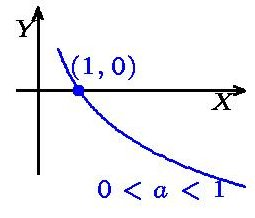
\includegraphics{logaritmischeB.jpg}
                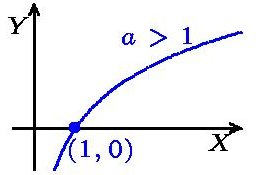
\includegraphics{logaritmischeA.jpg}
		\item \textcolor{green}{\hypertarget{logaritmen}{Formules}}\label{logaritmen}\newline
			\begin{itemize}
			\item[*] Gevolg van de definitie:
			\[\mbox{log}_a \:a^y =y\:\: \mbox{ en }\:\: a^{\mbox{log}_a \:x}=x\]
			\item[*] Logaritme van een product.
			\[\forall x_1, x_2, x_3 \in \R^+_0 : \mbox{log}_a\:(x_1 \cdot x_2\cdot x_3) = 			\mbox{log}_a \:x_1 + \mbox{log}_a \:x_2 + \mbox{log}_a \:x_3 \]
			\item[*] Logaritme van een quoti\"ent.
			\[\forall x_1, x_2 \in \R^+_0 : \mbox{log}_a\:(\ds\Frac {x_1}{x_2}) = 			\mbox{log}_a \:x_1 - \mbox{log}_a \:x_2 \]
			\item[*] Logaritme van een macht.
			\[\forall x \in \R^+_0\:;\: \forall r \in \R \: : \:\mbox{log}_a \:x^r 			= r\:\mbox{log}_a \:x\]
			\item[*] Verandering van grondtal.
			\[\mbox{log}_b \:x =\ds\Frac{\mbox{log}_a\:x}{\mbox{log}_a \:b}\]
			\end{itemize}
		 
		\end{itemize}%logaritmische functies


\hypertarget{bijzondere_functies}{}
\subsubsection{Grafieken van enkele bijzondere functies} \label{bijzondere_functies}

\begin{itemize}
\item[*] \textcolor{green}{\hypertarget{absolute_waardefunctie}{Absolute waardefunctie: $y=|\,x\,|$}} \label{absolute_waardefunctie}
  \begin{center}
  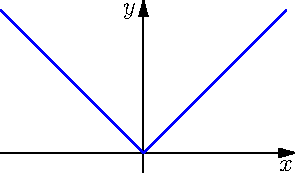
\includegraphics{absolute_waarde}
  \end{center}
\item[*] \textcolor{green}{Geheelfunctie (\hypertarget{trapfunctie}{trapfunctie}): $y=\lfloor\,x\,\rfloor$} \label{trapfunctie}\newline
  Dit is een functie waarbij $\lfloor\,x\,\rfloor$ het grootste geheel getal voorstelt kleiner dan of gelijk aan $x$.
  \begin{center}
  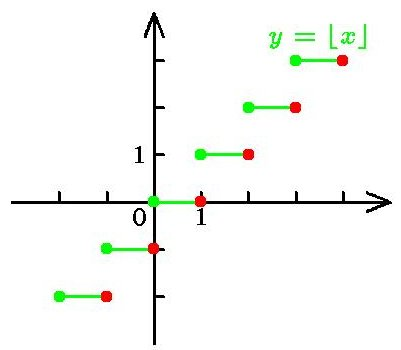
\includegraphics{trap.jpg}
  \end{center}
\item[*] \textcolor{green}{De functie \hypertarget{vierkantswortel}{$y=\sqrt{x}$}} \label{vierkantswortel}
  \begin{center}
  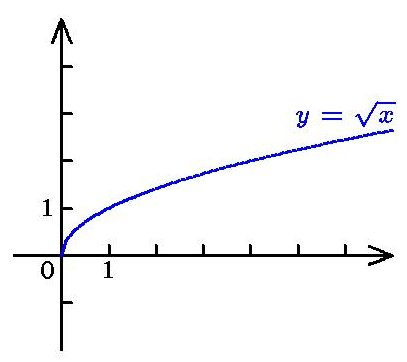
\includegraphics{vierkantswortel.jpg}
  \end{center}
\end{itemize}


% Dit werk is gelicenseerd onder een Creative Commons
% Naamsvermelding-GelijkDelen 3.0 Unported.
% Bezoek http://creativecommons.org/licenses/by-sa/3.0/ om een kopie te zien 
% van de licentie of stuur een brief naar Creative Commons, 444 Castro Street, 
% Suite 900, Mountain View, California, 94041, USA.

\section{GETALLEN} \label{getallen}
\hypertarget{getallen}{}

\subsection{Rijen} \label{rijen}
\hypertarget{rijen}{}
	\begin{enumerate}%Rijen
		\item \hypertarget{rekenkundige_rijen}{{\bf Rekenkundige rijen}}\label{rekenkundige_rijen}
		\begin{itemize}%rekenkundige rijen
		\item \textcolor{green}{Wat?}\newline
		Een rekenkundige rij is een rij waarbij elke term de {\bf som} is van de vorige term 		en een constant getal. Dit constant getal noemen we het {\it verschil} van de rij.
		\item \textcolor{green}{Voorbeelden.}\newline
		$1, 3, 5, 7, 9, \ldots$\newline
		$100, 90, 80, 70, 60, \ldots$
		\item \textcolor{green}{Formules.}\newline
			\begin{itemize}
			\item[*]	Algemene term.\newline
			Stel $t_n$ de $n$-de term van de rij en $v$ het verschil.
			\[t_n=t_{n-1}+v\]
			\[t_n=t_1+ (n-1)v\]
			\item[*] \hypertarget{rekenkundig_gemiddelde}{Rekenkundig gemiddelde}.\label{rekenkundig gemiddelde}\newline
			\begin{tabular}{c}
			 a, b,\:\mbox{en}\: c \:\mbox {zijn opeenvolgende termen van een 			rekenkundige rij}\\
			$\Updownarrow$ \\
			$b = \ds\Frac{a+c}{2}$
			\end{tabular}\vskip 0.5cm
			{\bf Eigenschap:} In een rekenkundige rij met een oneven aantal termen is 			de middelste term gelijk aan het rekenkundig gemiddelde van alle termen.
			\vskip 0.5cm
			\item[*] \hypertarget{som_rekenkundige_rij}{Som van de $n$ termen van een {\bf eindige} rekenkundige rij $(s_n)$:}
			\label{som rekenkundige rij}\newline
			\[s_n=n\ds\Frac{t_1+t_n}{2}\]
			\item[*] Toepassing: som van de eerste $n$ van nul verschillende natuurlijke 			getallen.
			\[ s_n = n \ds \Frac{n+1}{2}\]
			\end{itemize}
		\end{itemize}%rekenkundige rijen
		\item \hypertarget{meetkundige_rijen}{{\bf Meetkundige rijen}}\label{meetkundige_rijen}
		\begin{itemize}%meetkundige rijen
		\item \textcolor{green}{Wat?}\newline
		Een meetkundige rij is een rij waarbij elke term het {\bf product} is van de vorige 		term en een constant getal. Dit constant getal noemen we de {\it reden} van de rij.
		\item \textcolor{green}{Voorbeeld.}\newline
		$1, 2, 4, 8, 16, \ldots$ \newline
		$2, 3, \ds\Frac{9}{2}, \ds\Frac{27}{4},\ds\Frac{81}{8},\ldots$
		\item \textcolor{green}{Formules.}\newline
		\begin{itemize}
		\item[*] Algemene term.\newline
		Stel $t_n$ de $n$-de term van de rij en $r$ de reden.
		\[t_n = t_{n-1}\cdot r\]
		\[t_n = t_1 \cdot r^{n-1}\]
		\item[*] Meetkundig gemiddelde.\newline
		\begin{tabular}{c}
		 a, b,\:\mbox{en}\: c \:\mbox {zijn opeenvolgende termen van een meetkundige 		rij}\\
		$\Updownarrow$ \\
		$|b| = \sqrt{a \cdot c}$
		\end{tabular}
		\item[*] \hypertarget{som_meetkundige_rij}{Som van de $n$ termen van een {\bf eindige} meetkundige rij $(s_n)$:}
		\label{som meetkundige rij}\newline
		\[s_n=\ds\Frac{t_1(r^n-1)}{r-1}\]
		\item[*] Som van de termen van een convergerende meetkundige rij $(s)$:\newline
		Als $0 < |r| < 1$, dan convergeert de meetkundige rij en is de som van de termen:
		\[s = \ds\Frac{t_1}{1-r}\]		
		\end{itemize}
		\end{itemize}%meetkundige rijen
	\end{enumerate}%Rijen

\subsection{Machten met gehele exponenten} \label{machten_geheel}
\hypertarget{machten_geheel}{}
\begin{itemize}%machten geheel
\item {\bf met natuurlijke exponenten}
\begin{itemize}%natuurlijk
\item[*] \textcolor{green}{Definitie:} Zij $n \in \N$ en $a\in\R$, dan geldt: $a^n=\underbrace{a\cdot a\cdot a\cdot\ldots\cdot a}_{n\: keer}$
\item[*] \textcolor{green}{Afspraak:} $a^0=1$
\end{itemize}%natuurlijk
\item {\bf met gehele exponenten}
\begin{itemize}%geheel
\item[*] \textcolor{green}{Definitie:} Zij $n \in \N$ en $a \in \R_0$, dan geldt : $a^{-n}=\ds\Frac{1}{a^n}$
\end{itemize}%geheel
\item {\bf rekenregels voor machten met gehele exponenten}\newline
Zij $m, n \in \Z$ en $a, b \in \R_0$, dan geldt: \newline
\begin{eqnarray*}
a^m\cdot a^n & = & a^{m+n}\\
\ds\Frac{a^m}{a^n} & = & a^{m-n}\\
(a^m)^n & = & a^{mn}\\
a^m\cdot b^m & = & (a\cdot b)^m
\end{eqnarray*}
\end{itemize}%machten geheel

\subsection{$n$-de machtswortels} \label{wortelvormen}
\hypertarget{wortelvormen}{}
\begin{itemize}%wortelvormen
\item \textcolor{green}{Definitie}\newline
\begin{tabular}{c}
$w$ is een n-de machtswortel van $a$ \\
a.s.a\\
$w^n=a$
\end{tabular}\newline
\begin{itemize}
\item[*]Als $n$ {\bf even} is, heeft elk positief van 0 verschillend getal $a$ precies twee $n$-de machtswortels:\newline een positieve ($\sqrt[n]{a}$) en een negatieve ($-\sqrt[n]{a}$).\newline
\item[*]Als $n$ {\bf oneven} is, heeft elk getal \'e\'en $n$-de machtswortel ($\sqrt[n]{a}$) (kan positief of negatief zijn)
\end{itemize}
\item \textcolor{green}{Bestaansvoorwaarden}
\begin{itemize}%vwn
\item[*] {\bf $n$ even}\newline\newline
$\sqrt[n]{f(x)}$ bestaat $\Leftrightarrow \:f(x)\geq 0$ en $x$ behoort tot het domein van $f$\newline\newline
vb: $\sqrt[4]{x+1}$ bestaat $\Leftrightarrow \: x+1\geq 0 \:\Leftrightarrow\: x\geq -1$
\item[*] {\bf $n$ oneven}\newline\newline
$\sqrt[n]{f(x)}$ bestaat voor alle $x$ die tot het domein van $f$ behoren.\newline\newline
vb: $\sqrt[3]{x+1}$ bestaat voor alle $x \in \R$
\end{itemize}%vwn
\end{itemize}%wortelvormen

\subsection{Machten met re\"ele exponenten} \label{machten_reeel}
\hypertarget{machten_reeel}{}
\begin{itemize}%machten reeel
\item {\bf met gebroken rationale exponenten}
\begin{itemize}%gebroken
\item[*] \textcolor{green}{Definitie:} Zij $n \in \N_0, m \in \Z$ en $a \in \R_0^+$, dan geldt: $a^{\ds\Frac{m}{n}} = \sqrt[n]{a^m}$
\item[*] \textcolor{green}{Voorbeeld:} $8^{\ds\Frac{2}{3}}=\sqrt[3]{8^2}=4$
\end{itemize}%gebroken
\item {\bf met re\"ele exponenten}
\begin{itemize}%reeel
\item[*] \textcolor{green}{Voorbeeld:} $3^{\pi}$
\end{itemize}%reeel
\item {\bf rekenregels voor machten met re\"ele exponenten}\newline
Zij $r, s \in \R$ en $a, b \in \R_0^+$, dan geldt: \newline
\begin{eqnarray*}
a^s\cdot a^r & = & a^{s+r}\\
\ds\Frac{a^s}{a^r} & = & a^{s-r}\\
(a^s)^r & = & a^{sr}\\
a^s\cdot b^s & = & (a\cdot b)^s
\end{eqnarray*}
\end{itemize}%machten reeel

\subsection{Absolute waarde} \label{absolute_waarde}
\hypertarget{absolute_waarde}{}

\begin{itemize}
\item \textcolor{green}{Definitie:}
  \[
     |x| = \begin{cases}
            x & \Leftrightarrow x \in \R^+,\\
           -x & \Leftrightarrow x \in \R^-.
           \end{cases}
  \]
\item \textcolor{green}{Eigenschappen:}\newline
  \begin{itemize}
  \item[*] $|x|=0\ \Leftrightarrow\ x=0$
  \item[*] $|x\cdot y|=|x|\cdot|y|$
  \item[*] $|x|-|y|\leq |x+y|\leq |x|+|y|$
  \item[*] $a\in \R^+:|x| \leq a \ \Leftrightarrow\ -a\leq x \leq a$
  \item[*] $a\in\R^+:|x|>a \ \Leftrightarrow\ x> a$ \,of\, $x<-a$
  \end{itemize}
\end{itemize}

\subsection{Formules (merkwaardige producten, quoti\"enten...)} \label{formules}
\hypertarget{formules}{}
\begin{tabular}{l}
$(a\pm b)^2 = a^2\pm 2ab +b^2$\\\\
$(a\pm b)^3 = a^3\pm 3a^2b +3ab^2\pm b^3$\\\\
$a^2-b^2 = (a-b)(a+b)$\\\\
$a^3-b^3 = (a-b)(a^2+ab+b^2)$\\\\
$a^3+b^3 = (a+b)(a^2-ab+b^2)$\\\\
$a^4-b^4 = (a^2-b^2)(a^2+b^2)=(a-b)(a+b)(a^2+b^2)$\\
Of ook : $a^4-b^4=(a-b)(a^3+a^2b+ab^2+b^3)$\\\\
\end{tabular} \newline
Voor $(a+b)^5, (a+b)^6,\ldots$ zie binomium van Newton (\ref{binomium}).

\subsection{Deelbaarheid in $\Z$} \label{deelbaarheid}
\hypertarget{deelbaarheid}{}
\begin{itemize}%deelbaarheid
\item \textcolor{green}{Definitie:}
$\forall a, d \in \Z: d\,|\,a\ \Leftrightarrow\ \exists q\in \Z: a=dq$
\item \textcolor{green}{Stelling i.v.m. lineaire combinaties:}\newline
Zij $a,b,d \in \Z$\newline
$d\,|\,a$ en $d\,|\,b \ \Rightarrow\ d\,|\,xa+yb, \forall x, y \in \Z$
\item \textcolor{green}{Euclidische deling:}\newline
$\forall a \in \Z, b \in \N_0: \exists ! q\in \Z, \exists ! r \in \Z: a=bq+r$ met $0\leq r< b$
\item \textcolor{green}{Grootste gemene deler ggd$(a, b)$:}\newline
Zij $a, b \in \N_0$
\begin{eqnarray*}
\mbox{ggd}(a, b) & = & d\\
  & \Updownarrow & 
\end{eqnarray*}
\[ d \in \mbox{del}\,(a) \cap \mbox{del}\,(b) \mbox{ en } \forall c \in \mbox{del}\,(a) \cap \mbox{del} \,(b) : c \leq d \]\newline
{\bf Eigenschap:} De grootste gemene deler van twee van nul verschillende natuurlijke getallen is de kleinste positieve van nul verschillende lineaire combinatie met gehele co\"effici\"enten van die twee getallen.\vskip 0.5cm
\item \textcolor{green}{Kleinste gemeen veelvoud kgv$(a, b)$:}\newline
Zij $a, b, m \in \N_0$
\begin{eqnarray*}
\mbox{kgv}(a, b) & = & m\\
  & \Updownarrow & 
\end{eqnarray*}
\[ m \in a\Z \cap b\Z \mbox{ en } \forall c \in a\Z \cap b\Z \cap \N_0: c \geq m \]\newline
{\bf Eigenschap: } \[\mbox{kgv}(a, b)\cdot\mbox{ggd}(a, b)=a\cdot b\]
\item \textcolor{green}{Priemgetallen:}\newline
{\bf Definitie: }Zij $p \in \N$, dan is $p$ een priemgetal a.s.a. del$(p) \cap \N=\{1, p\}$.\newline
{\bf Eigenschap: } Elk natuurlijk getal, groter dan 1, is op unieke wijze te ontbinden in priemfactoren: \[n=p_1^{\alpha_1}p_2^{\alpha_2}p_3^{\alpha_3}\cdot\ldots\cdot p_q^{\alpha_q}\]
met $p_1, p_2, \ldots p_q$ priemgetallen en $\alpha_1, \alpha_2,\ldots\alpha_q \in \N_0$.\newline
{\bf Het aantal delers van een natuurlijk getal n} is dan $(\alpha_1+1)(\alpha_2+1)(\alpha_3+1)\cdot\ldots\cdot(\alpha_q+1)$.
\end{itemize}%deelbaarheid

\subsection{Complexe getallen} \label{complexe_getallen}
\hypertarget{complexe_getallen}{}
\begin{enumerate}%complexe getallen
\item \hypertarget{vorm_a_plus_bi}{{\bf De vorm $a + bi$}}\label{vorm_a_plus_bi}\vskip 0.3cm
\textcolor{green}{Eigenschappen en begrippen:}\newline
\begin{itemize} %vorm a+bi
\item[*] $i^2=-1$
\item[*] Als $z=a+bi$ dan is $\bar{z}=a-bi$ het complex toegevoegde. \newline
		Er geldt:
		\[\bar{z_1+z_2}=\bar{z_1}+\bar{z_2}\]
		\[\bar{z_1\cdot z_2}=\bar{z_1}\cdot\bar{z_2}\]
\end{itemize}%vorm a+bi
\item {\bf De goniometrische vorm}
\begin{itemize}
\item\textcolor{green}{Voorstelling in het complexe vlak:}\newline
%\docLink[tekening]{complexgetal.jpg}{\includegraphics{tekening.gif}}
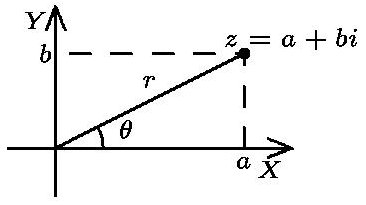
\includegraphics{complexgetal.jpg}
\item\textcolor{green}{\hypertarget{goniometrische_vorm}{Goniometrische vorm:}}\label{goniometrische_vorm}
		\[a+bi=r(\cos\theta +i\sin\theta)\]
\item\textcolor{green}{Product en quoti\"ent van twee complexe getallen:}\vskip 0.3 cm
Zij $z_1=r_1(\cos\theta_1 +i\sin\theta_1)$ en $z_2=r_2(\cos\theta_2+i\sin\theta_2)$.\vskip 0.3 cm Er geldt:
\[z_1\cdot z_2=r_1r_2(\cos(\theta_1+\theta_2)+i\sin(\theta_1+\theta_2)\] \vskip 0.3 cm
\[\ds\Frac{z_1}{z_2}=\ds\Frac{r_1}{r_2}(\cos(\theta_1-\theta_2)+i\sin(\theta_1-\theta_2)\]
\item\textcolor{green}{n-de macht van een complex getal:}\vskip 0.3 cm
\[\forall n\in \Z: (r(\cos\theta+i\sin\theta))^n=r^n(\cos n\theta + i\sin n\theta)\]\vskip 0.3 cm
\item\textcolor{green}{Formule van De Moivre:}
\[(\cos \theta +i\sin\theta)^n=\cos n\theta+i\sin n \theta\]\vskip 0.3 cm
\item\textcolor{green}{n-de machtswortels uit een complex getal $\:z=r(\cos\theta+i\sin\theta)$:}
\[\sqrt[n]{r}\cdot(\cos\ds\Frac{\theta+k\cdot 360^{\circ}}{n}+i\sin\ds\Frac{\theta+k\cdot360^{\circ}}{n})\: \mbox{met}\: k\in \Z\]
\end{itemize}\vskip 0.3 cm
\item \hypertarget{exponentiele_vorm}{{\bf Exponenti\"ele schrijfwijze van een complex getal $x+iy$}}\label{exponentiele_vorm}
\begin{itemize}%expon
\item \textcolor{green}{Formules}
\[x+iy=r e^{\theta i}=r(\cos\theta+i\sin\theta)\]
\[e^z=e^{x+iy}=e^x(\cos y+i\sin y)\]
\item \textcolor{green}{Gevolg}
\[\cos z =\ds\Frac{1}{2}(e^{zi}+e^{-zi})\]
\[\sin z =\ds\Frac{1}{2i}(e^{zi}-e^{-zi})\]
\end{itemize}%expon
\item \hypertarget{veeltermen_over_C}{{\bf Veeltermen over $\C$}}\label{veeltermen_over_C}
\begin{itemize}%veeltermen C
\item[*] Elke veelterm over $\C$ van de $n$-de graad heeft precies $n$ nulpunten in $\C$.
\item[*] Als het complexe getal $a+bi$ een nulpunt is van een veelterm met {\bf re\"ele} co\"effici\"enten, dan is ook het complex toegevoegde getal $a-bi$ een nulpunt van deze veelterm.
\end{itemize} %veeltermen C
\end{enumerate}%complexe getallen

\subsection{Statistiek} \label{statistiek}
\hypertarget{statistiek}{}
\begin{enumerate}%statistiek
\item\textcolor{green}{\hypertarget{begrippen}{Enkele begrippen:}}\label{begrippen}
\begin{itemize}% begrippen
\item {\it Populatie (universum)}: de verzameling van personen of objecten waarvan men 						kenmerk(en) wil onderzoeken
\item {\it Steekproef}: deelverzameling van de populatie, verzameling van die elementen van de 			populatie waarvoor de waarnemingen worden uitgevoerd.
\item {\it Variabele}: kenmerk dat men bij de elementen van de populatie wil nagaan. Aan de   				variabele worden waarden toegekend.  
\end{itemize}%begrippen
\item\textcolor{green}{\hypertarget{frequentietabel}{Frequentietabel:}}\label{frequentietabel}\newline
Stel $x_1, x_2, x_3, \ldots, x_n$ een steekproef met omvang $n$ en $p$ verschillende waarden.
\begin{center}
\begin{tabular}{|c|c|c|}
\hline
$x$ & absolute frequentie & relatieve frequentie\\ \hline
$x_1$ & $n_1$ & $f_1$ \\
$x_2$ & $n_2$ & $f_2$ \\
$\vdots$ & $ \vdots$ & $\vdots$\\
$x_p$ & $n_p$ & $f_p$ \\
\hline
\end{tabular}
\end{center}
\begin{itemize}
\item \hypertarget{absolute_frequentie}{{\bf Absolute frequentie:}}\label{absolute_frequentie} $n_i$ is het aantal keer dat de waarde $x_i$ voorkomt in de steekproef; er geldt:\vskip 0.5cm
\[\sum_{i=1}^{p}{n_i}=n\]
\item \hypertarget{relatieve_frequentie}{{\bf De relatieve frequentie:}}\label{relatieve_frequentie} $f_i=\ds\Frac{n_i}{n}$ en er geldt:
 \[\sum_{i=1}^{p}{f_i}=1\]
OF in procent: $f_i=\ds\Frac{n_i}{n}\cdot 100$ en er geldt:
\[\sum_{i=1}^{p}{f_i}=100\]
\end{itemize}
\item\textcolor{green}{\hypertarget{gemiddelde}{Gemiddelde($\bar{x}$):}}\label{gemiddelde}
\begin{itemize}
\item $\bar{x}=\Frac{1}{n}\sum_{i=1}^{p}{n_i\,x_i}$
\end{itemize}
Dit wordt ook wel {\it gewogen} gemiddelde genoemd.
\item\textcolor{green}{Variantie $(s^2)$ en \hypertarget{afwijking}{standaardafwijking $(s)$:}}\label{afwijking}
\begin{itemize}
\item $s^2=\ds\Frac{1}{n}\cdot\sum_{i=1}^{p}{n_i(x_i-\bar{x})^2}$
\item $s=\sqrt{\ds\Frac{1}{n}\cdot\sum_{i=1}^{p}{n_i(x_i-\bar{x})^2}}$
\end{itemize}
\end{enumerate}%statistiek


% Dit werk is gelicenseerd onder een Creative Commons
% Naamsvermelding-GelijkDelen 3.0 Unported.
% Bezoek http://creativecommons.org/licenses/by-sa/3.0/ om een kopie te zien 
% van de licentie of stuur een brief naar Creative Commons, 444 Castro Street, 
% Suite 900, Mountain View, California, 94041, USA.

\section{ALGEBRA} \label{algebra}
\hypertarget{algebra}{}

\subsection{Vergelijkingen} \label{vergelijkingen}
\hypertarget{vergelijkingen}{}

\subsubsection{Eerstegraadsvergelijkingen (lineaire vergelijkingen)} \label{eerstegraadsvergelijkingen}
\hypertarget{eerstegraadsvergelijkingen}{}
		\begin{itemize}%eerstegraadsvergelijkingen
		\item \textcolor{green}{Vorm.}
		\[ax+b=0, \: a\neq 0\]
		\item\textcolor{green}{Formule.}\newline
		Deze vergelijking heeft altijd \'e\'en oplossing: 
		\[x=-\ds\Frac{b}{a}\]
		\end{itemize}%eerstegraadsvergelijkingen

\subsubsection{Tweedegraadsvergelijkingen (vierkantsvergelijkingen)} \label{vierkantsvergelijkingen}
\hypertarget{vierkantsvergelijkingen}{}
		\begin{itemize}%tweedegraadsvergelijkingen
		\item \textcolor{green}{Vorm.}
		\[ax^2+bx+c=0, \: a\neq 0\]
		\item\textcolor{green}{Formules.}\newline
		Het aantal oplossingen hangt af van het teken van de discriminant ($D$):
		\[D=b^2-4ac\]
		Als $D>0$, dan zijn er twee verschillende oplossingen:
		\[x_{1,2}=\ds\Frac{-b\pm \sqrt{D}}{2a}\]
		Als $D=0$, dan zijn er twee gelijke oplossingen:
		\[x_1=x_2=\ds\Frac{-b}{2a}\]
		Als $D<0$, dan zijn er geen oplossingen.\newline\newline
		De \hypertarget{som_en_product}{{\bf som ($s$)} en het {\bf product ($p$)}} van de oplossingen:
		\label{som_en_product}
		\[s=-\ds\Frac{b}{a}\:\mbox{en}\:p=\ds\Frac{c}{a}\]\newline
		Een uitdrukking van de tweede graad ontbinden in factoren (als $D\geq 0$):\vskip 		0.5cm
		\[ax^2+bx+c=a(x-x_1)(x-x_2)\]met $x_1, x_2$ de oplossingen van de vergelijking
		$ax^2+bx+c=0$
		\end{itemize}%tweedegraadsvergelijkingen

\subsubsection{Bikwadratische vergelijkingen} \label{bikwadratische_vergelijkingen}
\hypertarget{bikwadratische_vergelijkingen}{}
		\begin{itemize}%bikwadratische vergelijkingen
		\item \textcolor{green}{Vorm.}
		\[ax^4+bx^2+c=0,\: a\neq 0\]
		\item \textcolor{green}{Methode.}\newline
		Door middel van een substitutie $t=x^2$ herleid je de bikwadratische vergelijking 		tot een vierkantsvergelijking in $t$. De gevonden oplossingen voor $t$ moet je 		daarna nog terug naar de variabele $x$ omzetten.
		\end{itemize}%bikwadratische vergelijkingen

\subsubsection{Vergelijkingen van de $n$-de graad} \label{n-de_graadsvergelijkingen}
\hypertarget{n-de_graadsvergelijkingen}{}
		\begin{itemize}%nde graadsvergelijkingen
		\item \textcolor{green}{Vorm.}
		\[a_nx^n+a_{n-1}x^{n-1}+\ldots +a_1x+a_0,\:\:a_n\neq 0\]
		\item \textcolor{green}{Methode.}\newline
		Probeer de $n$-de graadsuitdrukking te ontbinden in factoren, ofwel op het zicht ofwel via de methode van \hypertarget{horner}{{\bf Horner}}.\label{Horner}
		Volgens deze laatste zoek je een deler van de vorm $x-a$.
		\newline
		Criterium van deelbaarheid:
		\[x-a\: | \: f(x) \Leftrightarrow f(a)=0\]\newline
		Verder zoek je het quoti\"ent met het rekenschema van	{\bf 		Horner}.\newline\newline\newline
		\item \textcolor{green}{Voorbeeld.}\newline
		$\mbox{Los op:}\: x^3+2x^2-5x+2=0$\newline
		$f(1)=0 \: \Rightarrow\:  x-1 \: |\: f(x)$
		\[\begin{tabular}{l|lll|l}
		 & 1 & 2 & -5 & 2\\
		 &   &   &    &  \\
		1&   & 1 & 3  & -2\\
		\hline
		 & 1 & 3 & -2 & 0\\
		\end{tabular}\]
		Het quoti\"ent is dan $x^2+3x-2$, zodat we krijgen:
		\[(x-1)(x^2+3x-2)=0\]
		Verdere ontbinding levert:
		\[(x-1)(x-\ds\Frac{-3+\sqrt{17}}{2})(x+\ds\Frac{-		3+\sqrt{17}}{2})=0\]\newline
		De oplossingenverzameling is dan $\{1,\ds\Frac{-		3+\sqrt{17}}{2},\ds\Frac{-3-\sqrt{17}}{2} \}$\vskip 2cm
		\end{itemize}%nde graadsvergelijkingen

\subsubsection{Irrationale vergelijkingen} \label{irrationale_vergelijkingen}
\hypertarget{irrationale_vergelijkingen}{}
		Een irrationale vergelijking is een vergelijking waarbij de variabele $x$ onder het 		wortelteken voorkomt.\newline
		\textcolor{green} {Voorbeelden:}
		\[\sqrt{x+2}=x \hskip 3cm (1)\]
		\vskip 0.5cm
		\[\sqrt{x}=5-\sqrt{x+1}\hskip 2.2cm (2)\]
		De methode van oplossen bestaat erin te kwadrateren tot de vierkantswortels 		verdwenen zijn.\newline
		Er zijn wel enkele voorwaarden op te stellen: bestaansvoorwaarden en 		kwadrateringsvoorwaarden.\newline
		\textcolor{green}{De oplossingen:}\newline
		\[\sqrt{x+2}=x\]
		De bestaansvoorwaarde: \begin{eqnarray}
						x+2 & \geq &  0\\
						x & \geq & -2
						\end{eqnarray}
		De kwadrateringsvoorwaarde: \[x \geq 0\]
		De vergelijking wordt dan: \begin{eqnarray}
						   \sqrt{x+2}&=&x	\\
						   x+2 & = & x^2\\
						   x^2-x-2 & = 0\\
						   x=-1 & \mbox{of} & x=2		
						   \end{eqnarray}	
		De eerste oplossing voldoet niet aan de voorwaarden, de tweede wel, \newline 
		dus de oplossingenverzameling is $\{2\}$.\vskip 1cm
		\[\sqrt{x}=5-\sqrt{x+1}\]
		\[\sqrt{x}+\sqrt{x+1}=5\]
		De bestaansvoorwaarden: \begin{eqnarray}
						x & \geq &  0\\
						  &      &   \\
						  &      &   \\ 					
						x+1 & \geq &  0\\
						x & \geq & -1
						\end{eqnarray}
		De vergelijking wordt dan: \begin{eqnarray}
						   x+2\sqrt{x(x+1)}+x+1 & = & 25\\
						   2\sqrt{x(x+1)} & = & 24-2x\\
						   \sqrt{x(x+1)} & = & 12-x\\			
						   \end{eqnarray}	
		De kwadrateringsvoorwaarde: \begin{eqnarray}
						    12-x & \geq &  0\\
						    x & \leq & 12
						    \end{eqnarray}
		Verder krijgen we dan: \begin{eqnarray}
						x(x+1) & = & 144-24x+x^2\\
						x & = & \displaystyle\Frac{144}{25}
						\end{eqnarray}
		Deze oplossing voldoet aan alle voorwaarden, dus de oplossingenverzameling is 		$\{\displaystyle\Frac{144}{25}\}$.


% Dit werk is gelicenseerd onder een Creative Commons
% Naamsvermelding-GelijkDelen 3.0 Unported.
% Bezoek http://creativecommons.org/licenses/by-sa/3.0/ om een kopie te zien 
% van de licentie of stuur een brief naar Creative Commons, 444 Castro Street, 
% Suite 900, Mountain View, California, 94041, USA.

\section{GONIOMETRIE} \label{goniometrie}
\hypertarget{goniometrie}{}

\subsection{Goniometrische getallen van een hoek} \label{goniometrische_getallen}
\hypertarget{goniometrische_getallen}{}

\subsubsection{Hoofdwaarde van een hoek} \label{hoofdwaarde_hoek}

Als de hoekgrootte $\alpha$ is, dan zijn $\alpha + k\cdot 360\degree$, $k\in \mathbb{Z}$, ook waarden voor dezelfde hoek. De {\bf hoofdwaarde} is die waarde die behoort tot $]-180\degree,180\degree]$.

\subsubsection{In een rechthoekige driehoek} \label{rechthoekige_driehoek}
\hypertarget{rechthoekige_driehoek}{}

\begin{center}
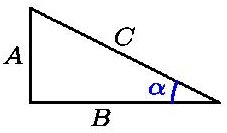
\includegraphics{rechtdriehoek.jpg}
\end{center}
\begin{eqnarray*}
\sin\alpha&=&\ds\Frac{A}{C}\\
\cos\alpha&=&\ds\Frac{B}{C}\\
\mbox{tg}\:\alpha&=&\ds\Frac{\sin\alpha}{\cos\alpha}=\ds\Frac{A}{B}\\
\mbox{cotg}\:\alpha&=&\ds\Frac{1}{\mbox{tg}\alpha}=\ds\Frac{B}{A}
\end{eqnarray*}

\subsubsection{De goniometrische cirkel} \label{goniometrische_cirkel}
\hypertarget{goniometrische_cirkel}{}

\begin{center}
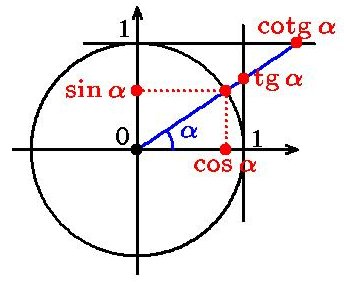
\includegraphics{goncirkel.jpg}
\end{center}

\subsubsection{Bijzondere hoeken} \label{bijzondere_hoeken}
\hypertarget{bijzondere_hoeken}{}

% todo: benamingen voor tg, cot, sec en csc zijn hier juist, maar in rest document anders (met mbox...)
\begin{center}
  \renewcommand{\arraystretch}{1.5}
  \begin{tabular}{c|ccccc}
    $\alpha$ & $0=0\degree$ & $\frac{\pi}{6}=30\degree$ & $\frac{pi}{4}=45\degree$ & $\frac{pi}{3}=60\degree$ & $\frac{pi}{2}=90\degree$\\
    \hline
    $\sin\alpha$ & $0$ & $\frac{1}{2}$ & $\frac{\sqrt{2}}{2}$ & $\frac{\sqrt{3}}{2}$ & $1$\\
    $\cos\alpha$ & $1$ & $\frac{\sqrt{3}}{2}$ & $\frac{\sqrt{2}}{2}$ & $\frac{1}{2}$ & $0$\\
    $\tan\alpha$ & $0$ & $\frac{1}{\sqrt{3}}$ & $1$ & $\sqrt{3}$ & $\infty$\\
    $\cot\alpha$ & $\infty$ & $\sqrt{3}$ & $1$ & $\frac{1}{\sqrt{3}}$ & $0$\\
    $\sec\alpha$ & $1$ & $\frac{2}{\sqrt{3}}$ & $\sqrt{2}$ & $2$ & $\infty$\\
    $\csc\alpha$ & $\infty$ & $2$ & $\sqrt{2}$ & $\frac{\sqrt{2}}{3}$ & $1$\\
  \end{tabular}
\end{center}

Om het goniometrische getal van een hoek in het tweede, derde of vierde kwadrant te vinden herleidt je deze hoek eerst naar een hoek van het eerste kwadrant met de formules van verwante hoeken (zie verder).

\subsubsection{Formules} \label{goniometrische_formules}
\hypertarget{goniometrische_formules}{}

\begin{itemize}
\item \textcolor{green}{Grondformule en afgeleide formules}
\begin{eqnarray*}
\ds\Frac{1}{\sin\alpha} & = & \mbox{cosec}\alpha\\
\ds\Frac{1}{\cos\alpha} & = & \mbox{sec}\alpha\\
\cos^2\alpha+\sin^2\alpha&=&1\\
1+\:\mbox{tg}^2\alpha &=&\:\mbox{sec}^2\alpha\\
1+\:\mbox{cotg}^2\alpha&=&\:\mbox{cosec}^2\alpha
\end{eqnarray*}
\item \textcolor{green}{\hypertarget{verwante_hoeken}{Verwante hoeken}}\label{verwante hoeken}
	\begin{itemize}%verwante hoeken
	\item[*] Tegengestelde hoeken ($\alpha$ en $-\alpha$)
	\begin{eqnarray*}
	\sin(-\alpha)& =&-\sin\alpha\\
	\cos(-\alpha)&=&\cos\alpha\\
	\mbox{tg}\:(-\alpha)&=&-\:\mbox{tg}\:\alpha\\
	\mbox{cotg}\:(-\alpha)&=&-\:\mbox{cotg}\:\alpha
	\end{eqnarray*}
	\item[*] Supplementaire hoeken ($\alpha$ en $\pi-\alpha$)
	\begin{eqnarray*}
	\sin(\pi-\alpha)& =&\sin\alpha\\
	\cos(\pi-\alpha)&=&-\cos\alpha\\
	\mbox{tg}\:(\pi-\alpha)&=&-\:\mbox{tg}\:\alpha\\
	\mbox{cotg}\:(\pi-\alpha)&=&-\:\mbox{cotg}\:\alpha
	\end{eqnarray*}
	\item[*] Complementaire hoeken ($\alpha$ en $\ds\Frac{\pi}{2}-\alpha$)
	\begin{eqnarray*}
	\sin(\ds\Frac{\pi}{2}-\alpha)& =&\cos\alpha\\
	\cos(\ds\Frac{\pi}{2}-\alpha)&=&\sin\alpha\\
	\mbox{tg}\:(\ds\Frac{\pi}{2}-\alpha)&=&\:\mbox{cotg}\:\alpha\\
	\mbox{cotg}\:(\ds\Frac{\pi}{2}-\alpha)&=&\:\mbox{tg}\:\alpha
	\end{eqnarray*}
	\item[*] Antisupplementaire hoeken ($\alpha$ en $\pi+\alpha$)
	\begin{eqnarray*}
	\sin(\pi+\alpha)& =&-\sin\alpha\\
	\cos(\pi+\alpha)&=&-\cos\alpha\\
	\mbox{tg}\:(\pi+\alpha)&=&\:\mbox{tg}\:\alpha\\
	\mbox{cotg}\:(\pi+\alpha)&=&\:\mbox{cotg}\:\alpha
	\end{eqnarray*}
	\item[*] Anticomplementaire hoeken ($\alpha$ en $\ds\Frac{\pi}{2}+\alpha$)
	\begin{eqnarray*}
	\sin(\ds\Frac{\pi}{2}+\alpha)& =&\cos\alpha\\
	\cos(\ds\Frac{\pi}{2}+\alpha)&=&-\sin\alpha\\
	\mbox{tg}\:(\ds\Frac{\pi}{2}+\alpha)&=&-\:\mbox{cotg}\:\alpha\\
	\mbox{cotg}\:(\ds\Frac{\pi}{2}+\alpha)&=&-\:\mbox{tg}\:\alpha
	\end{eqnarray*}
	\end{itemize}%verwante hoeken
\item \textcolor{green}{\hypertarget{som-en_verschilformules}{Som- en verschilformules}}\label{som-en_verschilformules}
\begin{eqnarray*}
\cos(\alpha-\beta)&=&\cos\alpha\,\cos\beta+\sin\alpha\,\sin\beta\\
\cos(\alpha+\beta)&=&\cos\alpha\,\cos\beta-\sin\alpha\,\sin\beta\\	
\sin(\alpha+\beta)&=&\sin\alpha\,\cos\beta+\cos\alpha\,\sin\beta\\
\sin(\alpha-\beta)&=&\sin\alpha\,\cos\beta-\cos\alpha\,\sin\beta\\
\mbox{tg}\:(\alpha+\beta)&=&\ds\Frac{\mbox{tg}\:\alpha+\:\mbox{tg}\:\beta}{1-	\:\mbox{tg}\:\alpha\:\mbox{tg}\:\beta}\\
\mbox{tg}\:(\alpha-\beta)&=&\ds\Frac{\mbox{tg}\:\alpha-	\:\mbox{tg}\:\beta}{1+	\:\mbox{tg}\:\alpha\:\mbox{tg}\:\beta}
\end{eqnarray*}
\item \textcolor{green}{\hypertarget{simpson}{Formules van Simpson}}\label{simpson}
\begin{eqnarray*}
\sin\alpha+\sin\beta&=&2\sin\ds\Frac{\alpha+\beta}{2}\,\cos\ds\Frac{\alpha-\beta}{2}\\
\sin\alpha-\sin\beta&=&2\cos\ds\Frac{\alpha+\beta}{2}\,\sin\ds\Frac{\alpha-\beta}{2}\\
\cos\alpha+\cos\beta&=&2\cos\ds\Frac{\alpha+\beta}{2}\,\cos\ds\Frac{\alpha-\beta}{2}\\
\cos\alpha-\cos\beta&=&-2\sin\ds\Frac{\alpha+\beta}{2}\,\sin\ds\Frac{\alpha-\beta}{2}\\
\end{eqnarray*}
\item \textcolor{green}{\hypertarget{dubbele_hoek}{Formules voor de dubbele hoek}}\label{dubbele_hoek}
\begin{eqnarray*}
\sin(2\alpha)&=&2\sin\alpha\,\cos\alpha\\
\cos(2\alpha)&=&\cos^2\alpha - \sin^2\alpha\\
\mbox{tg}(2\alpha)&=&\ds\Frac{2\:\mbox{tg}\:\alpha}{1-\:\mbox{tg}^2\alpha}
\end{eqnarray*}
\item \textcolor{green}{\hypertarget{t-formules}{t-formules}}\label{t-formules}\newline
Stel $\mbox{tg}\Frac{\alpha}{2}=t$, dan kunnen we $\sin\alpha, \cos\alpha$ en 	$\mbox{tg}\,\alpha$ schrijven in functie van $t$.
\begin{eqnarray*}
\sin\alpha&=&\Frac{2t}{1+t^2}\\
\cos\alpha&=&\Frac{1-t^2}{1+t^2}\\
\mbox{tg}\,\alpha&=&\Frac{2t}{1-t^2}
\end{eqnarray*}
\end{itemize}

\subsubsection{Oplossen van driehoeken} \label{oplossen_driehoeken}
\hypertarget{oplossen_driehoeken}{}
	\begin{itemize}%oplossen van drhn
	\item \textcolor{green}{Rechthoekige driehoeken}
		\begin{itemize}%rechthoekige drhn
		\item[*]De stelling van Pythagoras:
		\[C^2=A^2+B^2\]
		\end{itemize}%rechthoekige drhn
	\item \textcolor{green}{Willekeurige driehoeken}\newline
		%\docLink[tekening]{driehoek.jpg}{\includegraphics{tekening.gif}}
                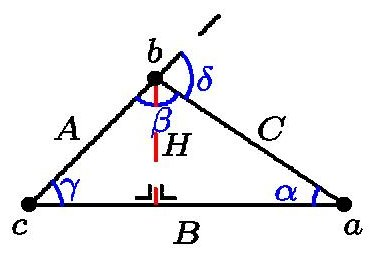
\includegraphics{driehoek.jpg}
		\begin{itemize}%willekeurige drhn
		\item[*] De \hypertarget{sinusregel}{{\bf sinusregel}}:\label{sinusregel}
		\[\ds\Frac{A}{\sin\alpha}=\ds\Frac{B}{\sin\beta}=\ds\Frac{C}{\sin\gamma}=2R\]
		met $R$ de straal van de omgeschreven cirkel.\newline
		\item[*] De \hypertarget{cosinusregel}{{\bf cosinusregel}}:\label{cosinusregel}
		\begin{eqnarray*}
		A^2&=&B^2+C^2-2BC\cos\alpha\\
		B^2&=&A^2+C^2-2AC\cos\beta\\
		C^2&=&A^2+B^2-2AB\cos\gamma
		\end{eqnarray*}
		\end{itemize}%willekeurige drhn
	\end{itemize}%oplossen van drhn


\subsection{Goniometrische functies}

Zie Sectie~\ref{goniometrische_functies} op pagina~\pageref{goniometrische_functies}.


% Dit werk is gelicenseerd onder een Creative Commons
% Naamsvermelding-GelijkDelen 3.0 Unported.
% Bezoek http://creativecommons.org/licenses/by-sa/3.0/ om een kopie te zien 
% van de licentie of stuur een brief naar Creative Commons, 444 Castro Street, 
% Suite 900, Mountain View, California, 94041, USA.

\section{VLAKKE MEETKUNDE} \label{vlakke meetkunde}
\hypertarget{vlakke_meetkunde}{}

\subsection{Stelling van Thales} \label{thales}
\hypertarget{thales}{}
De lijnstukken ingesneden door evenwijdige rechten op een snijlijn zijn evenredig met de overeenkomende lijnstukken ingesneden op elke andere snijlijn.
\[\ds\Frac{|ab|}{|bc|}=\ds\Frac{|a'b'|}{|b'c'|}\]
%\docLink[tekening]{thales.jpg}{\includegraphics{tekening.gif}}\newline
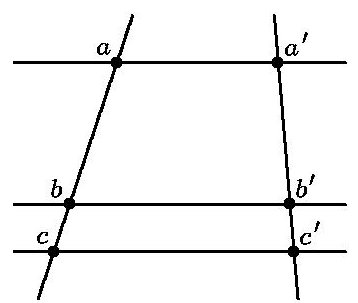
\includegraphics{thales.jpg}
In het bijzonder geldt bij evenwijdige projectie:
De projecties van evenwijdige lijnstukken hebben dezelfde verhouding als de lijnstukken zelf.

\subsection{Driehoeken} \label{driehoeken}
\hypertarget{driehoeken}{}

%\docLink[tekening]{driehoek.jpg}{\includegraphics{tekening.gif}}
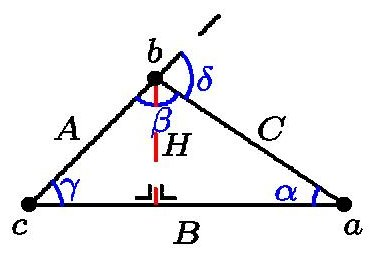
\includegraphics{driehoek.jpg}

\subsubsection{Oppervlakte (O)} \label{oppervlakte driehoek}
\hypertarget{oppervlakte_driehoek}{}
	\[O=\ds\Frac{B\cdot H}{2}\]
	Of ook:\newline\label{alternatief}
	\begin{eqnarray*}
	O &=&\ds\Frac{1}{2}\cdot A\cdot B\cdot \sin\gamma \\
	  &=&\ds\Frac{1}{2}\cdot B\cdot C\cdot \sin\alpha \\
	  &=&\ds\Frac{1}{2}\cdot C\cdot A\cdot \sin\beta \\
	\end{eqnarray*}

\subsubsection{Eigenschappen} \label{eigenschappen}
\hypertarget{eigenschappen}{}
		\begin{itemize}%eign
		\item De {\bf som van de hoeken} van een driehoek is 	$180^{\circ}$.
		\[\alpha+\beta+\gamma=180^{\circ}\]
		\item Een \hypertarget{buitenhoek}{{\bf buitenhoek}} \label{buitenhoek} van een driehoek is gelijk aan de som 		van de niet-aanliggende binnenhoeken.
		\[\delta=\alpha+\gamma\]
		\item In een rechthoekige driehoek geldt de stelling van \hypertarget{pythagoras}{{\bf Pythagoras}}: 		\label{Pythagoras} \[C^2=A^2+B^2\] met $C$ de schuine zijde en $A, B$ de 		rechthoekzijden.
		\end{itemize}%eign

\subsubsection{Merkwaardige lijnen} \label{merkwaardige_lijnen}
\hypertarget{merkwaardige_lijnen}{}
		\begin{itemize}%merkw lijnen
		\item \hypertarget{zwaartelijn}{{\bf Zwaartelijnen $(Z_a, Z_b, Z_c)$}}\label{zwaartelijn}\newline
		De drie zwaartelijnen gaan door \'e\'en punt, het zwaartepunt.\newline\newline
		{\bf Eigenschap v.h. zwaartepunt:}het zwaartepunt verdeelt de zwaartelijnen in twee 		stukken waarvan de lengtes zich verhouden als 2 en 1.
		\[|m_az|=\ds\Frac{1}{2}|za|\]
		%\docLink[tekening]{zwaartelijnen.jpg}{\includegraphics{tekening.gif}}
                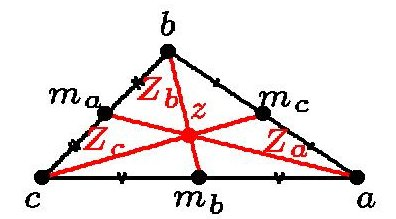
\includegraphics{zwaartelijnen.jpg}
		\item \hypertarget{hoogtelijn}{{\bf Hoogtelijnen $(H_a, H_b, H_c)$}}\label{hoogtelijn}\newline
		De drie hoogtelijnen gaan door \'e\'en punt.\newline
		%\docLink[tekening]{hoogtelijnen.jpg}{\includegraphics{tekening.gif}}
                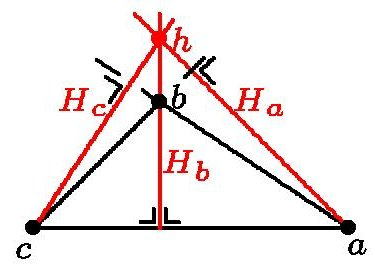
\includegraphics{hoogtelijnen.jpg}
		\item \hypertarget{{\bf Bissectrices of deellijnen $(D_a, D_b, D_c)$}}\label{bissectrice}\newline
		De drie bissectrices gaan door \'e\'en punt dat bovendien het middelpunt is van de 		ingeschreven cirkel.\newline
		%\docLink[tekening]{bissectrices.jpg}{\includegraphics{tekening.gif}}
                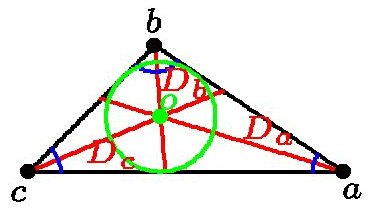
\includegraphics{bissectrices.jpg}
		\item \hypertarget{middelloodlijn}{{\bf Middelloodlijnen $(M_1, M_2, M_3)$}}\label{middelloodlijn}\newline
		De drie middelloodlijnen gaan door \'e\'en punt dat bovendien het middelpunt is van 		de omgeschreven cirkel.\newline
		%\docLink[tekening]{middelloodlijnen.jpg}{\includegraphics{tekening.gif}}
                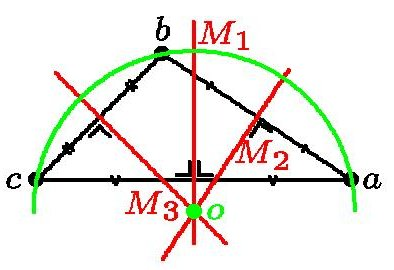
\includegraphics{middelloodlijnen.jpg}
		\end{itemize}%merkw lijnen

\subsubsection{De middenparallel} \label{middenparallel}
\hypertarget{middenparallel}{}
		De {\bf middenparallel} van een driehoek is het lijnstuk dat de middens van twee 		zijden verbindt. Een driehoek heeft er drie. Er geldt bovendien: $|m_1m_2| = 		\ds\Frac{1}{2}|ac|$\newline
		%\docLink[tekening]{middenparallel.jpg}{\includegraphics{tekening.gif}}
                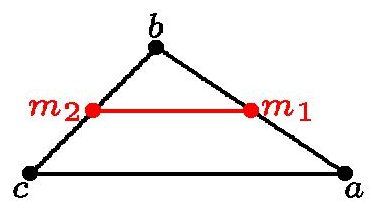
\includegraphics{middenparallel.jpg}

\subsubsection{Congruente driehoeken} \label{congruente_driehoeken}
\hypertarget{congruente_driehoeken}{}
		\begin{itemize}%congruent
		\item \hypertarget{congruente_veelhoeken}{{\bf Definitie congruente veelhoeken:}} \label{congruente_veelhoeken} Congruente veelhoeken 		zijn veelhoeken die door verplaatsing in elkaar kunnen overgaan m.a.w. die elkaar 		volledig kunnen bedekken.
		\item {\bf Gevallen van congruentie bij driehoeken}
			\begin{itemize}%gevallen v. congr.
			\item[*] Twee driehoeken zijn congruent als ze \'e\'en zijde en twee hoeken 			gelijk hebben.
			\item[*] Twee driehoeken zijn congruent als ze twee zijden en de ingesloten 			hoek gelijk hebben.
			\item[*] Twee driehoeken zijn congruent als ze de drie zijden gelijk hebben.
			\end{itemize}%gevallen v. congr.
		\end{itemize}%congruent

\subsubsection{Gelijkvormige driehoeken} \label{gelijkvormige_driehoeken}
\hypertarget{gelijkvormige_driehoeken}{}
		\begin{itemize}%gelijkvormig
		\item {\bf Definitie gelijkvormige veelhoeken:} Gelijkvormige veelhoeken zijn 		veelhoeken die gelijke hoeken hebben en waarvan de overeenkomstige zijden evenredig 		zijn.\newline
		{\bf Gevolg:}\newline\newline
		\begin{tabular}{c}
		$\triangle{abc} \sim \triangle{a'b'c'}$\\
				 $\Updownarrow$ 	\\
            $\ds\Frac{|ab|}{|a'b'|}=\Frac{|bc|}{|b'c'|}=\Frac{|ca|}{|c'a'|}$ \\ 		\end{tabular}		
		\item {\bf Gevallen van gelijkvormigheid bij driehoeken}
			\begin{itemize}%gevallen gelijkv.
			\item[*] Twee driehoeken zijn gelijkvormig als ze twee hoeken gelijk hebben.
			\item[*] Twee driehoeken zijn gelijkvormig als twee zijden van de ene evenredig 			zijn met twee zijden van de andere en de ingesloten hoeken gelijk zijn.
			\item[*] Twee driehoeken zijn gelijkvormig als de drie zijden van de ene 			evenredig zijn met de drie zijden van de andere.
			\item[*] Twee driehoeken zijn gelijkvormig als de zijden van de ene evenwijdig 			lopen met of loodrecht staan op de zijden van de andere.
			\end{itemize}%gevallen gelijkv
		\end{itemize}%gelijkvormig

\subsubsection{Driehoeksongelijkheid} \label{driehoeksongelijkheid}
\hypertarget{driehoeksongelijkheid}{}

%\docLink[tekening]{driehoeksongelijkheid.jpg}{\includegraphics{tekening.gif}}\newline
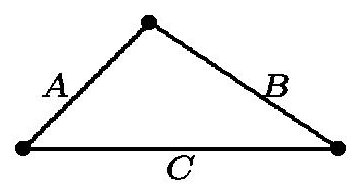
\includegraphics{driehoeksongelijkheid.jpg}
		Zij $A, B$ en $C$ de lengtes van de zijden van een driehoek ($A\:\leq\: B\leq 		C$), dan geldt:
		\[C-B\:\leq \:A\leq B+C\]
		\[C-A\:\leq \:B\leq A+C\]
		\[B-A\:\leq C\:\leq B+A\]

\subsection{Vierhoeken} \label{vierhoeken}
\hypertarget{vierhoeken}{}

\subsubsection{Parallellogram} \label{parallellogram}
\hypertarget{parallellogram}{}
		\begin{itemize}%par
		\item[*]{\bf Definitie:} Een parallellogram is een vierhoek waarvan de 		overstaande zijden evenwijdig zijn.\newline
		%\docLink[tekening]{parallellogram.jpg}{\includegraphics{tekening.gif}}
                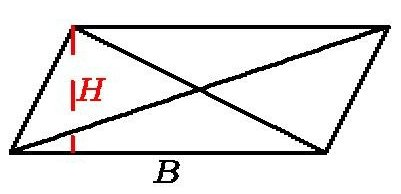
\includegraphics{parallellogram.jpg}
		\item[*]{\bf Oppervlakte (O):} $O = B\cdot H$
		\item[*]{\bf Eigenschap:} De diagonalen snijden elkaar middendoor.
		\item[*]{\bf Speciale gevallen:}
			\begin{itemize}
			\item[$\bullet$]Een {\bf ruit} is een vierhoek met vier gelijke 			zijden.\newline
			{\bf Eigenschap:} De diagonalen staan loodrecht op elkaar en delen de 			hoeken middendoor.
			%\docLink[tekening]{ruit.jpg}{\includegraphics{tekening.gif}}
                        \includegraphics{ruit.jpg}
			\item[$\bullet$]Een {\bf rechthoek} is een vierhoek met vier gelijke 			hoeken.\newline 
			{\bf Eigenschap:} De diagonalen zijn gelijk.\newline
			%\docLink[tekening]{rechthoek.jpg}{\includegraphics{tekening.gif}}
                        \includegraphics{rechthoek.jpg}
			\item[$\bullet$]Een {\bf vierkant} is een rechthoek met vier gelijke 			zijden.\newline
			%\docLink[tekening]{vierkant.jpg}{\includegraphics{tekening.gif}}
                        \includegraphics{vierkant.jpg}
			\end{itemize}
		\end{itemize}%par

\subsubsection{Trapezium} \label{trapezium}
\hypertarget{trapezium}{}
		\begin{itemize}%trap 
		\item[*]{\bf Definitie:}
		Een trapezium is een vierhoek met twee evenwijdige zijden.
		\item[*]{\bf Oppervlakte (O):} $O=\ds\Frac{b+B}{2}\cdot H$
		\item[*]{\bf Middenparallel:}$|m_1m_2|=\ds\Frac{b+B}{2}$
		\end{itemize}%trap
		%\docLink[tekening]{trapezium.jpg}{\includegraphics{tekening.gif}}
                \includegraphics{trapezium.jpg}

\subsection{Veelhoeken} \label{veelhoeken}
\hypertarget{veelhoeken}{}
	\begin{itemize}%veelh
	\item De som van de hoeken van een n-hoek is gelijk aan: $(n-2)180^{\circ}$
	\item Elke hoek van een {\bf regelmatige n-hoek} is gelijk aan: $\ds\Frac{(n-	2)180^{\circ}}{n}$
	\end{itemize}%veelh

\subsection{Cirkels} \label{cirkels}
\hypertarget{cirkels}{}
Zij $r$ de straal van de cirkel.\newline

\subsubsection{Omtrek:} \label{omtrek_cirkel}
\hypertarget{omtrek_cirkel}{}
$2\pi r$ 

\subsubsection{Oppervlakte:}\label{oppervlakte_cirkel}
\hypertarget{oppervlakte_cirkel}{}
$\pi r^2$

\subsubsection{Raaklijn-normaal} \label{raaklijn-normaal}
\hypertarget{raaklijn-normaal}{}
	\begin{itemize}
	\item[*] Een {\bf raaklijn} aan een cirkel is een rechte die juist \'e\'en punt gemeen 	heeft met de cirkel.
	\item[*] Een raaklijn aan een cirkel staat loodrecht op de straal naar het raakpunt.
	\item[*] De {\bf normaal} in een punt op de cirkel is de loodlijn in dit punt op de 	raaklijn.
	\end{itemize}

\subsubsection{Boog-koorde} \label{boog-koorde}
\hypertarget{boog-koorde}{}
	\begin{itemize}
	\item[*]Een {\bf boog} is een deel van de cirkelomtrek.
	\item[*]{\bf Lengte van een \hypertarget{cirkelboog}{cirkelboog}:} $\alpha r$\label{cirkelboog}\newline
	\item[*]Een {\bf koorde} is een lijnstuk dat de eindpunten van een boog verbindt.
	\end{itemize}
	%\docLink[tekening]{cirkel.jpg}{\includegraphics{tekening.gif}}
        \includegraphics{cirkel.jpg}

\subsubsection{Middelpuntshoek-omtrekshoek} \label{middelpunts-omtrekshoek}
\hypertarget{middelpunts-omtrekshoek}{}
	\begin{itemize}
	\item[*] Een {\bf omtrekshoek} meet de {\bf helft} van de middelpuntshoek op dezelfde 	boog.
	\item[*] Omtrekshoeken die op eenzelfde boog staan, zijn gelijk.
	\end{itemize}
	%\docLink[tekening]{omtrekshoek.jpg}{\includegraphics{tekening.gif}}
        \includegraphics{omtrekshoek.jpg}

\subsubsection{Binnen- en buitenomtrekshoek} \label{binnen-buitenomtrekshoek} 
\hypertarget{binnen-buitenomtrekshoek}{}
	\begin{itemize}
	\item[*] Een {\bf binnenomtrekshoek} heeft hetzelfde maatgetal als de halve {\bf som} van 	de boog binnen de hoek en de boog binnen de overstaande hoek.
	\[\alpha=\ds\Frac{1}{2}(\stackrel{\frown}{ab}+\stackrel{\frown}{cd})\]
	%\docLink[tekening]{binnenomtrk.jpg}{\includegraphics{tekening.gif}}
        \includegraphics{binnenomtrk.jpg}
	\item[*] Een {\bf buitenomtrekshoek} heeft hetzelfde maatgetal als het halve {\bf 	verschil} van de bogen binnen de hoek. 
	\[\alpha=\ds\Frac{1}{2}(\stackrel{\frown}{ab}-\stackrel{\frown}{cd})\]
	%\docLink[tekening]{buitenomtrk.jpg}{\includegraphics{tekening.gif}}
        \includegraphics{buitenomtrk.jpg}
	\end{itemize}

\subsubsection{Sector-segment} \label{sector-segment}
\hypertarget{sector-segment}{}
	\begin{itemize}
	\item[*]Een {\bf cirkelsegment} is de figuur gevormd door een boog en zijn koorde.\newline
	%\docLink[tekening]{segment.jpg}{\includegraphics{tekening.gif}}
        \includegraphics{segment.jpg}
	\item[*]Een \hypertarget{sector}{{\bf cirkelsector}} is de figuur gevormd door een boog en de stralen naar zijn eindpunten.\label{sector}\newline
	%\docLink[tekening]{sector.jpg}{\includegraphics{tekening.gif}}
        \includegraphics{sector.jpg}
	\item[*] {\bf Oppervlakte van een cirkelsector:} $\ds\Frac{1}{2}\alpha r^2$
	\end{itemize}

\subsubsection{Macht van een punt t.o.v. de cirkel} \label{macht_punt-cirkel}
\hypertarget{macht_punt-cirkel}{}
	Het product van de afstanden van een punt $p$ tot de snijpunten van een veranderlijke 	rechte door $p$ met de cirkel, is constant; die constante noemen we de {\bf macht van 	het punt tot de cirkel}.
	\[|pa|\cdot|pb|=|pc|\cdot|pd|\]
	%\docLink[tekening]{macht.jpg}{\includegraphics{tekening.gif}}
        \includegraphics{macht.jpg}

\subsubsection{Koordenvierhoek} \label{koordenvierhoek}
\hypertarget{koordenvierhoek}{}
	\begin{itemize}
	\item[*]Een {\bf koordenvierhoek} is een vierhoek ingeschreven in een cirkel.
	\item[*]In een koordenvierhoek zijn de overstaande hoeken $\alpha$ en $\beta$ elkaars 	supplement.
	\end{itemize}
	%\docLink[tekening]{koordenvierhoek.jpg}{\includegraphics{tekening.gif}}
        \includegraphics{koordenvierhoek.jpg}

\subsection{Analytische meetkunde} \label{analytische_meetkunde}
\hypertarget{analytische_meetkunde}{}

\subsubsection{Afstand tussen twee punten} \label{afstand_twee_punten}
\hypertarget{afstand_twee_punten}{}
Zij $p(x_1, y_1)$ en $q(x_2, y_2)$ twee punten dan geldt:\newline
\[d(p, q)=|pq|=\sqrt{(x_2-x_1)^2+(y_2-y_1)^2}\]

\subsubsection{Midden van een lijnstuk} \label{midden_lijnstuk}
\hypertarget{midden_lijnstuk}{}
Zij $a(x_1, y_1)$ en $b(x_2, y_2)$ twee punten in het vlak, dan is de co\"ordinaat van het midden $(m)$ van het lijnstuk $[ab]$:
\[co(m)=\left(\ds\Frac{x_1+x_2}{2}, \ds\Frac{y_1+y_2}{2}\right)\]

\subsubsection{Afstand van een punt tot een rechte} \label{afstand_punt-rechte}
\hypertarget{afstand_punt-rechte}{}
Zij $A\:\leftrightarrow\:ax+by+c=0$ een rechte en $p(x_1, x_2)$ een punt, dan geldt:\newline
\[d(p, A)=\ds\Frac{|ax_1+by_1+c|}{\sqrt{a^2+b^2}}\]
De \hypertarget{normaalvergelijking}{{\bf normaalvergelijking}} van een rechte $L\,\leftrightarrow\,ax +by+c=0$ is:\label{normaalvergelijking}
\[\ds\Frac{ax+by+c}{\sqrt{a^2 + b^2}}=0\]

\subsubsection{Loodrechte stand - evenwijdigheid} \label{loodrecht-evenwijdig}
\hypertarget{loodrecht-evenwijdig}{}
\begin{itemize}
\item[*]Twee rechten met respectieve richtingsco\"effici\"enten $m_1$ en $m_2$ staan {\bf loodrecht} op elkaar a.s.a $m_1m_2=-1$.
\item[*]Twee rechten met respectieve richtingsco\"effici\"enten $m_1$ en $m_2$ zijn {\bf evenwijdig} a.s.a. $m_1=m_2$.
\end{itemize}

\subsubsection{De vergelijking van de cirkel} \label{vergelijking_cirkel}
\hypertarget{vergelijking_cirkel}{}
Zij $m(x_1,y_1)$ het middelpunt en $r$ de straal van de cirkel, dan is de (middelpunts)vergelijking:
\[C(m, r)\:\leftrightarrow\:(x-x_1)^2+(y-y_1)^2=r^2\]

\subsection{Vectoren} \label{vectoren}
\hypertarget{vectoren}{}

\subsubsection{Definitie:} \label{definitie}
\hypertarget{definitie}{}
{\bf Vector $\vec{ab}$} is de verzameling van alle lijnstukken die dezelfde lengte, richting en 
zin hebben als het geori\"enteerde lijnstuk $\vec{ab}$.\newline
Grafisch wordt $\vec{ab}$ voorgesteld door \'e\'en representant van die verzameling.\newline
%\docLink[tekening]{vectoren1.jpg}{\includegraphics{tekening.gif}}\newline
\includegraphics{vectoren1.jpg}
Met {\bf plaatsvector} $\vec{p}$ wordt vector $\vec{op}$ bedoeld, met $o$ de oorsprong van het vlak.\newline
%\docLink[tekening]{vectoren2.jpg}{\includegraphics{tekening.gif}}
\includegraphics{vectoren2.jpg}

\subsubsection{Co\"ordinaat van een vector (componentenkoppel)} \label{coordinaten}
\hypertarget{coordinaten}{}
Bij plaatsvectoren geldt: co$(\vec{p})=co(p)=(x_1, x_2)$\newline
De co\"ordinaat van $\vec{ab}$ is dezelfde als die van zijn plaatsvector.\newline
%\docLink[tekening]{vectoren3.jpg}{\includegraphics{tekening.gif}}
\includegraphics{vectoren3.jpg}

\subsubsection{Optellen van vectoren} \label{optellen_vectoren}
\hypertarget{optellen_vectoren}{}
Voor het optellen van vectoren geldt de regel van het parallellogram.\newline
%\docLink[tekening]{vectoren4.jpg}{\includegraphics{tekening.gif}}\newline
\includegraphics{vectoren4.jpg}
Met co\"ordinaten: als co$(\vec{V})=(x_1, y_1)$ en co($\vec{W})=(x_2, y_2)$ dan is:
\[co(\vec{V}+\vec{W})=(x_1 +x_2, y_1+y_2)\]

\subsubsection{Scalaire vermenigvuldiging} \label{scalaire_vermenigv}
\hypertarget{scalaire_vermenigv}{}
Het $r$-voud van een vector $\vec{V}$ is een vector met lengte $|r|$ maal de lengte van $\vec{V}$, richting dezelfde als die van $\vec{V}$ en zin dezelfde als die van $\vec{V}$ (r>0) of tegengesteld aan die van $\vec{V}$ (r<0).\newline
Met co\"ordinaten: als co$(\vec{V})=(x_1, y_1)$, dan is:
\[co(r\vec{V})=(rx_1, ry_1)\]

\subsubsection{Norm van een vector} \label{norm_vector}
\hypertarget{norm_vector}{}
De norm van een vector: $\|\vec{ab}\|$ is de afstand d$(a, b)$.\newline
Met co\"ordinaten: als co$(\vec{V})=(x_1, y_1)$ dan is:
\[\|\vec{V}\| = \sqrt{x_1^2 + y_1^2}\]

\subsubsection{Ongelijkheid van Minkowski} \label{minkowski}
\hypertarget{minkowski}{}
\[\|\vec{V}+\vec{W}\|\, \leq\, \|\vec{V}\| + \|\vec{W}\|\]

\subsubsection{Hoek tussen twee vectoren} \label{hoek_vectoren}
\hypertarget{hoek_vectoren}{}

Als $\vec{U}$ en $\vec{V}$ verschillend zijn van $\vec{0}$, co($\vec{U})=(x_1, y_1)$ en co($\vec{V})=(x_2, y_2)$ en $\varphi$ de hoek tussen beide vectoren, dan is: 
\[cos(\varphi)=\ds\Frac{x_1x_2+y_1y_2}{\sqrt{x_1^2+y_1^2}\cdot\sqrt{x_2^2+y_2^2}}\]

\subsubsection{Scalair product van twee vectoren} \label{scalair_product_vectoren}
\hypertarget{scalair_product_vectoren}{}
Als $\vec{U}$ en $\vec{V}$ verschillend zijn van $\vec{0}$ en $\varphi$ de hoek is tussen beide vectoren, dan is het scalair product:
\[\vec{U}\cdot \vec{V} = \|\vec{U}\|\cdot\|\vec{V}\|\cdot \mbox{cos}(\varphi)\]
Met co\"ordinaten: 
\[\vec{U}\cdot\vec{V}=x_1x_2+y_1y_2\]

\subsubsection{Orthogonaliteit van vectoren:} \label{orthogonaliteit_vectoren}
\hypertarget{orthogonaliteit_vectoren}{}
Twee vectoren $\vec{U}$ en $\vec{V}$ zijn orthogonaal als $\vec{U}\cdot \vec{V}=0$.


% Dit werk is gelicenseerd onder een Creative Commons
% Naamsvermelding-GelijkDelen 3.0 Unported.
% Bezoek http://creativecommons.org/licenses/by-sa/3.0/ om een kopie te zien 
% van de licentie of stuur een brief naar Creative Commons, 444 Castro Street, 
% Suite 900, Mountain View, California, 94041, USA.

\section{RUIMTEMEETKUNDE} \label{ruimtemeetkunde}
\hypertarget{ruimtemeetkunde}{}

\subsection{Inhoud en oppervlakte van ruimtefiguren} \label{inhoud_ruimtefiguren}
\hypertarget{inhoud_ruimtefiguren}{}

\subsubsection{Prisma} \label{prisma}
\hypertarget{prisma}{}
Stel $G$ de oppervlakte van het grondvlak.\newline
%\docLink[tekening]{prisma.jpg}{\includegraphics{tekening.gif}}\newline
\includegraphics{prisma.jpg}
$I=G\cdot h$

\subsubsection{Piramide} \label{piramide}
\hypertarget{piramide}{}
Stel $G$ de oppervlakte van het grondvlak.\newline
%\docLink[tekening]{piramide.jpg}{\includegraphics{tekening.gif}}\newline
\includegraphics{piramide.jpg}
$I=\ds\Frac{1}{3}G\cdot h$

\subsubsection{Cilinder} \label{cilinder}
\hypertarget{cilinder}{}
%\docLink[tekening]{cilinder.jpg}{\includegraphics{tekening.gif}}\newline
\includegraphics{cilinder.jpg}
$I=\pi r^2 h$\newline
De zijdelingse oppervlakte van een rechte cilinder: $O = 2\pi r h $

\subsubsection{Kegel} \label{kegel}
\hypertarget{kegel}{}
%\docLink[tekening]{kegel.jpg}{\includegraphics{tekening.gif}}\newline
\includegraphics{kegel.jpg}
$I=\ds\Frac{1}{3}\pi r^2 h$\newline
De zijdelingse oppervlakte van een rechte kegel: $O = \pi r \sqrt{h^2+r^2}$

\subsubsection{Bol} \label{bol}
\hypertarget{bol}{}
%\docLink[tekening]{bol.jpg}{\includegraphics{tekening.gif}}\newline
\includegraphics{bol.jpg}
$I=\ds\Frac{4}{3}\pi r^3$\newline
De oppervlakte: $O = 4\pi r^2$

\subsection{Vectoren}
Zie hoofdstuk over vectoren in Sectie~\ref{vectoren} op pagina~\pageref{vectoren}.

\subsection{Co\"ordinaten in de ruimte} \label{coordinaten_in_de_ruimte}
\hypertarget{coordinaten_in_de_ruimte}{}

\subsubsection{Richtingsvectoren-richtingsgetallen} \label{richtingsgetallen}
\hypertarget{richtingsgetallen}
\[\vec{pq} \,\mbox{is een {\bf richtingsvector} van de rechte}\, A \,\Leftrightarrow\, pq \| A\]
\vskip 0.5cm
\begin{center}
De co\"ordinaat van een richtingsvector van A noemen we een stel {\bf richtingsgetallen} van A.
\end{center}
\vskip 0.5cm
{\bf Voorbeeld:} \newline Zij $p(x_1, y_1, z_1)$ en $q(x_2, y_2, z_2)$ twee punten gelegen op de rechte A.\newline Dan is $\vec{pq}$ een richtingsvector van A en is co$(\vec{pq})=(x_2-x_1, y_2-y_1, z_2-z_1)$ een stel richtingsgetallen van $A$.

\subsubsection{Vergelijkingen van een rechte} \label{vergelijking_rechte}
\hypertarget{vergelijking_rechte}{}
\begin{itemize}
\item[*] Rechte bepaald door punt en richtingsvector:\vskip 0.5cm
Zij $p(x_1, y_1, z_1)$ een punt van de rechte en $\vec{q}(a_1, b_1, c_1)$ een richtingsvector, dan zijn de {\bf parametervergelijkingen}:
\begin{eqnarray*}
x & = & x_1 +ra_1 \\
y & = & y_1 +rb_1 \\
z & = & z_1 +rc_1 \\
\end{eqnarray*}
en de {\bf Cartesiaanse vergelijkingen }: 
\[\ds\Frac{x-x_1}{a_1}=\Frac{y-y_1}{b_1}=\Frac{z-z_1}{c_1}\]\vskip 0.5cm
\item[*] Rechte bepaald door twee punten:\vskip 0.5 cm
Zij $p(x_1, y_1, z_1)$ en $q(x_2, y_2, z_2)$ twee punten van de rechte, dan zijn de {\bf parametervergelijkingen}:
\begin{eqnarray*}
x=x_1+r(x_2-x_1)\\
y=y_1+r(y_2-y_1)\\
z=z_1+r(z_2-z_1)\\
\end{eqnarray*}
en de {\bf Cartesiaanse vergelijkingen}: 
\[\ds\Frac{x-x_1}{x_2-x_1}=\Frac{y-y_1}{y_2-y_1}=\Frac{z-z_1}{z_2-z_1}\]
\end{itemize}

\subsubsection{Vergelijking van een vlak} \label{vergelijking_vlak}
\hypertarget{vergelijking_vlak}{}
\begin{itemize}
\item[*] Vlak bepaald door een punt en twee onafhankelijke richtingsvectoren:\vskip 0.5 cm
Zij $p(x_1, y_1, z_1)$ een punt en $\vec{q}(a_1, b_1, c_1)$ en $\vec{r}(a_2, b_2, c_2)$ twee onafhankelijke richtingsvectoren van het vlak, dan is de {\bf parametervoorstelling}:
\begin{eqnarray*}
x=x_1+ka_1+la_2\\
y=y_1+kb_1+lb_2\\
z=z_1+kc_1+lc_2\\
\end{eqnarray*}
\item[*] {\bf Cartesiaanse vergelijking} van een vlak:
\[ux+vy+wz+t=0\] met $u, v, w, t \in \R$ en $\vec{n}\,(u, v, w)$ een normaalvector van dat vlak.
(Een normaalvector van een vlak is een vector die loodrecht staat op het vlak.) 
\item[*] {\bf Determinantvergelijking} van een vlak:\vskip 0.5 cm
Zij $p(x_1, y_1, z_1)$ een punt en $q(a_1, b_1, c_1)$ en $r(a_2, b_2, c_2)$ twee onafhankelijke richtingsvectoren van het vlak, dan is de determinantvergelijking:
\begin{eqnarray*}\left|\begin{array}{cccc}
		x & y & z & 1 \\
		x_1 & y_1 & z_1 & 1 \\
		a_1 & b_1 & c_1 & 0 \\
		a_2 & b_2 & c_2 & 0 \\
			\end{array} \right| & = & 0 \\
\end{eqnarray*}
Zij $p_1(x_1, y_1, z_1)$, $p_2(x_2, y_2, z_2)$ en $p_3(x_3, y_3, z_3)$ drie punten van het vlak, dan is de determinantvergelijking:
\begin{eqnarray*}\left|\begin{array}{cccc}
		x & y & z & 1 \\
		x_1 & y_1 & z_1 & 1 \\
		x_2 & y_2 & z_2 & 1 \\
		x_3 & y_3 & z_3 & 1 \\
		\end{array} \right| & = & 0\\
\end{eqnarray*}
\end{itemize}

\subsubsection{Middelpuntsvergelijking van een bol} \label{vergelijking_bol}
\hypertarget{vergelijking_bol}{}
Zij $\Sigma (m, r)$ een bol met middelpunt $m(x_1, y_1, z_1)$ en straal $r$, dan is de middelpuntsvergelijking:
\[\Sigma (m, r) \leftrightarrow (x-x_1)^2 + (y-y_1)^2 + (z-z_1)^2=r^2\]

\subsubsection{Cartesiaanse vergelijkingen van omwentelingslichamen} \label{vergelijking_omwentelingslichamen}
\hypertarget{vergelijking_omwentelingslichamen}{}
\begin{itemize}
\item[*] Bol met middelpunt in de oorsprong:\vskip 0.5cm
$\Sigma \,\leftrightarrow\, x^2+y^2+z^2=r^2$\newline
%\docLink[tekening]{bolanal.jpg}{\includegraphics{tekening.gif}}
\includegraphics{bolanal.jpg}
\item[*] Cilindervlak met rotatieas de Z-as:\vskip 0.5cm
$\mathcal{C} \,\leftrightarrow\, x^2+y^2=r^2$\newline
%\docLink[tekening]{cilinderanal.jpg}{\includegraphics{tekening.gif}}
\includegraphics{cilinderanal.jpg}
\item[*] Kegelvlak met rotatieas de Z-as:\vskip 0.5cm
$\mathcal{K} \,\leftrightarrow\, x^2+y^2=(z-h)^2tg^2\alpha$\newline
%\docLink[tekening]{kegelanal.jpg}{\includegraphics{tekening.gif}}
\includegraphics{kegelanal.jpg}
\item[*] Hyperbolo\"ide:\newline
\[\mathcal{H} \,\leftrightarrow\, x^2+y^2-z^2=1\]
\item[*] Parabolo\"ide:\newline
\[\mathcal{P}\, \leftrightarrow\, x^2+y^2=4z\]
%\includegraphics{para_klein.gif}
\end{itemize}


% Dit werk is gelicenseerd onder een Creative Commons
% Naamsvermelding-GelijkDelen 3.0 Unported.
% Bezoek http://creativecommons.org/licenses/by-sa/3.0/ om een kopie te zien 
% van de licentie of stuur een brief naar Creative Commons, 444 Castro Street, 
% Suite 900, Mountain View, California, 94041, USA.

\section{LOGICA} \label{logica}
\hypertarget{logica}{}

\subsection{Verklaring van de gebruikte symbolen} \label{verklaring_symbolen}
\hypertarget{verklaring_symbolen}{}
In wat volgt worden volgende symbolen gebruikt:\vskip 0.5cm
\begin{tabular}{l|l}
symbool & verklaring \\
\hline
$P, Q, R$ & uitspraken \\
$\neg$ & niet \\
$\vee$ & of \\
$\wedge$ & en \\
$\Rightarrow$ & als...dan \\
$\Leftrightarrow$ & als en slechts als \\
$\forall$ & voor alle\\
$\exists$ & er bestaat\\
\end{tabular}\vskip 0.5cm

\subsection{Logische stellingen} \label{logische_stellingen}
\hypertarget{logische_stellingen}{}
\begin{enumerate}%logische stellingen
\item $\neg(\neg P)\:\Leftrightarrow\: P$
\item $(P\:\Rightarrow\: Q) \:\Leftrightarrow\: (\neg P \vee Q)$
\item $((P \:\Rightarrow\: Q)\wedge P)\:\Rightarrow\: Q$
\item $((P \:\Rightarrow\: Q)\wedge \neg Q)\:\Rightarrow\: \neg P$
\item $(\neg(P \:\wedge\: Q)\wedge P)\:\Rightarrow\: \neg Q$
\item $(P \vee Q)\wedge\neg Q)\:\Rightarrow\:P$
\item \textcolor{green}{Contrapositie van de implicatie:}$(P\:\Rightarrow\: Q) \:\Leftrightarrow\: (\neg Q \:\Rightarrow\: \neg P)$
\item \textcolor{green}{\hypertarget{de_morgan}{Wetten van De Morgan:}}\label{de_morgan}\newline
\begin{tabular}{c}
$\neg(P\wedge Q)\:\Leftrightarrow\:\neg P \vee \neg Q $\\
$\neg(P \vee Q)\:\Leftrightarrow\:\neg P \wedge \neg Q$
\end{tabular}
\item \textcolor{green}{Commutativiteiten:}\newline
\begin{tabular}{rcl}
$P \wedge Q$ & $\Leftrightarrow $ & $Q \wedge P$\\
$P \vee Q$ & $\Leftrightarrow $ & $Q \vee P$\\
$(P \:\Leftrightarrow\: Q)$ & $\Leftrightarrow $ & $(Q \:\Leftrightarrow\: P$)\\
\end{tabular}
\item \textcolor{green}{Associativiteiten:}\newline
\begin{tabular}{rcl}
$(P \wedge Q)\wedge R$ & $\Leftrightarrow $ & $P \wedge (Q \wedge R)$\\
$(P \vee Q)\vee R$ & $\Leftrightarrow $ & $P \vee (Q \vee R)$\\
$((P \:\Leftrightarrow\: Q)\:\Leftrightarrow\: R)$ & $\Leftrightarrow $ & $(P\:\Leftrightarrow\: (Q \:\Leftrightarrow\: R))$\\
\end{tabular}
\item \textcolor{green}{Distributiviteiten:}\newline
\begin{tabular}{rcl}
$P \wedge (Q\vee R)$ & $\Leftrightarrow $ & $(P \wedge Q) \vee (P\wedge R)$\\
$P \vee (Q\wedge R)$ & $\Leftrightarrow $ & $(P \vee Q) \wedge (P\vee R)$\\
\end{tabular}
\item \textcolor{green}{Transitiviteiten:}\newline
\begin{tabular}{rcl}
$((P \:\Rightarrow\: Q)\wedge (Q\:\Rightarrow\: R))$ & $ \Rightarrow $ & $(P \:\Rightarrow\: R)$ \\
$((P \:\Leftrightarrow\: Q)\wedge (Q\:\Leftrightarrow\: R))$ & $ \Rightarrow $ & $(P \:\Leftrightarrow\: R)$ \\
\end{tabular}
\end{enumerate}%logische stellingen
\vskip 0.5cm

\subsection{Uitspraakvormen met kwantoren} \label{uitspraakvormen_kwantoren}
\hypertarget{uitspraakvormen_kwantoren}{}
Stel $P(x)$ een uitspraakvorm in de veranderlijke $x$ en $A$ een referentieverzameling.\newline Dan gelden volgende wetten:\vskip 0.5cm
\begin{tabular}{rcl}
$\neg(\forall x \in A:P(x)) $ & $\Leftrightarrow$ & $\exists\: x \in A: \neg P(x)$\\
$\neg(\exists x \in A:P(x)) $ & $\Leftrightarrow$ & $\forall\: x \in A: \neg P(x)$\\
\end{tabular}


% Dit werk is gelicenseerd onder een Creative Commons
% Naamsvermelding-GelijkDelen 3.0 Unported.
% Bezoek http://creativecommons.org/licenses/by-sa/3.0/ om een kopie te zien 
% van de licentie of stuur een brief naar Creative Commons, 444 Castro Street, 
% Suite 900, Mountain View, California, 94041, USA.


\vspace{2em}
\noindent\fbox{\begin{minipage}{\textwidth}\begin{center}\includegraphics{by-sa.png}\end{center}Dit werk is gelicenseerd onder een Creative Commons Naamsvermelding-GelijkDelen 3.0 Unported. Bezoek http://creativecommons.org/licenses/by-sa/3.0/ om een kopie te zien van de licentie of stuur een brief naar Creative Commons, 444 Castro Street, Suite 900, Mountain View, California, 94041, USA.\end{minipage}}

\end{document}

% Dit werk is gelicenseerd onder een Creative Commons
% Naamsvermelding-GelijkDelen 3.0 Unported.
% Bezoek http://creativecommons.org/licenses/by-sa/3.0/ om een kopie te zien 
% van de licentie of stuur een brief naar Creative Commons, 444 Castro Street, 
% Suite 900, Mountain View, California, 94041, USA.
